%%%%%%%%%%%%%%%%%%%%%%%%%%%%%%%%%%%%%%%%%
% Lachaise Assignment
% LaTeX Template
% Version 1.0 (26/6/2018)
%
% This template originates from:
% http://www.LaTeXTemplates.com
%
% Authors:
% Marion Lachaise & François Févotte
% Vel (vel@LaTeXTemplates.com)
%
% License:
% CC BY-NC-SA 3.0 (http://creativecommons.org/licenses/by-nc-sa/3.0/)
% 
%%%%%%%%%%%%%%%%%%%%%%%%%%%%%%%%%%%%%%%%

%----------------------------------------------------------------------------------------
%	PACKAGES AND OTHER DOCUMENT CONFIGURATIONS
%----------------------------------------------------------------------------------------

\documentclass{article}

%%%%%%%%%%%%%%%%%%%%%%%%%%%%%%%%%%%%%%%%%
% Lachaise Assignment
% Structure Specification File
% Version 1.0 (26/6/2018)
%
% This template originates from:
% http://www.LaTeXTemplates.com
%
% Authors:
% Marion Lachaise & François Févotte
% Vel (vel@LaTeXTemplates.com)
%
% License:
% CC BY-NC-SA 3.0 (http://creativecommons.org/licenses/by-nc-sa/3.0/)
% 
%%%%%%%%%%%%%%%%%%%%%%%%%%%%%%%%%%%%%%%%%

%----------------------------------------------------------------------------------------
%	PACKAGES AND OTHER DOCUMENT CONFIGURATIONS
%----------------------------------------------------------------------------------------

\usepackage{amsmath,amsfonts,stmaryrd,amssymb,float,graphicx,enumerate,mathtools,listings,xcolor,color,esint,subfig,tikz,pgfplots,setspace,graphicx,array,longtable} % Math packages

\usepackage{enumerate} % Custom item numbers for enumerations

\usepackage[ruled]{algorithm2e} % Algorithms

\usepackage[framemethod=tikz]{mdframed} % Allows defining custom boxed/framed environments

\usepackage{listings} % File listings, with syntax highlighting
\lstset{
	basicstyle=\ttfamily, % Typeset listings in monospace font
}

%----------------------------------------------------------------------------------------
%	DOCUMENT MARGINS
%----------------------------------------------------------------------------------------

\usepackage{geometry} % Required for adjusting page dimensions and margins

\geometry{
	paper=a4paper, % Paper size, change to letterpaper for US letter size
	top=2.5cm, % Top margin
	bottom=3cm, % Bottom margin
	left=2.5cm, % Left margin
	right=2.5cm, % Right margin
	headheight=14pt, % Header height
	footskip=1.5cm, % Space from the bottom margin to the baseline of the footer
	headsep=1.2cm, % Space from the top margin to the baseline of the header
	%showframe, % Uncomment to show how the type block is set on the page
}

%----------------------------------------------------------------------------------------
%	FONTS
%----------------------------------------------------------------------------------------

\usepackage[utf8]{inputenc} % Required for inputting international characters
\usepackage[T1]{fontenc} % Output font encoding for international characters

\usepackage{XCharter} % Use the XCharter fonts

%----------------------------------------------------------------------------------------
%	COMMAND LINE ENVIRONMENT
%----------------------------------------------------------------------------------------

% Usage:
% \begin{commandline}
%	\begin{verbatim}
%		$ ls
%		
%		Applications	Desktop	...
%	\end{verbatim}
% \end{commandline}

\mdfdefinestyle{commandline}{
	leftmargin=10pt,
	rightmargin=10pt,
	innerleftmargin=15pt,
	middlelinecolor=black!50!white,
	middlelinewidth=2pt,
	frametitlerule=false,
	backgroundcolor=black!5!white,
	frametitle={Command Line},
	frametitlefont={\normalfont\sffamily\color{white}\hspace{-1em}},
	frametitlebackgroundcolor=black!50!white,
	nobreak,
}

% Define a custom environment for command-line snapshots
\newenvironment{commandline}{
	\medskip
	\begin{mdframed}[style=commandline]
}{
	\end{mdframed}
	\medskip
}

%----------------------------------------------------------------------------------------
%	FILE CONTENTS ENVIRONMENT
%----------------------------------------------------------------------------------------

% Usage:
% \begin{file}[optional filename, defaults to "File"]
%	File contents, for example, with a listings environment
% \end{file}

\mdfdefinestyle{file}{
	innertopmargin=1.6\baselineskip,
	innerbottommargin=0.8\baselineskip,
	topline=false, bottomline=false,
	leftline=false, rightline=false,
	leftmargin=2cm,
	rightmargin=2cm,
	singleextra={%
		\draw[fill=black!10!white](P)++(0,-1.2em)rectangle(P-|O);
		\node[anchor=north west]
		at(P-|O){\ttfamily\mdfilename};
		%
		\def\l{3em}
		\draw(O-|P)++(-\l,0)--++(\l,\l)--(P)--(P-|O)--(O)--cycle;
		\draw(O-|P)++(-\l,0)--++(0,\l)--++(\l,0);
	},
	nobreak,
}

% Define a custom environment for file contents
\newenvironment{file}[1][File]{ % Set the default filename to "File"
	\medskip
	\newcommand{\mdfilename}{#1}
	\begin{mdframed}[style=file]
}{
	\end{mdframed}
	\medskip
}

%----------------------------------------------------------------------------------------
%	NUMBERED QUESTIONS ENVIRONMENT
%----------------------------------------------------------------------------------------

% Usage:
% \begin{question}[optional title]
%	Question contents
% \end{question}

\mdfdefinestyle{question}{
	innertopmargin=1.2\baselineskip,
	innerbottommargin=0.8\baselineskip,
	roundcorner=5pt,
	nobreak,
	singleextra={%
		\draw(P-|O)node[xshift=1em,anchor=west,fill=white,draw,rounded corners=5pt]{%
		Question \theQuestion\questionTitle};
	},
}

\newcounter{Question} % Stores the current question number that gets iterated with each new question

% Define a custom environment for numbered questions
\newenvironment{question}[1][\unskip]{
	\bigskip
	\stepcounter{Question}
	\newcommand{\questionTitle}{~#1}
	\begin{mdframed}[style=question]
}{
	\end{mdframed}
	\medskip
}

%----------------------------------------------------------------------------------------
%	WARNING TEXT ENVIRONMENT
%----------------------------------------------------------------------------------------

% Usage:
% \begin{warn}[optional title, defaults to "Warning:"]
%	Contents
% \end{warn}

\mdfdefinestyle{warning}{
	topline=false, bottomline=false,
	leftline=false, rightline=false,
	nobreak,
	singleextra={%
		\draw(P-|O)++(-0.5em,0)node(tmp1){};
		\draw(P-|O)++(0.5em,0)node(tmp2){};
		\fill[black,rotate around={45:(P-|O)}](tmp1)rectangle(tmp2);
		\node at(P-|O){\color{white}\scriptsize\bf !};
		\draw[very thick](P-|O)++(0,-1em)--(O);%--(O-|P);
	}
}

% Define a custom environment for warning text
\newenvironment{warn}[1][Warning:]{ % Set the default warning to "Warning:"
	\medskip
	\begin{mdframed}[style=warning]
		\noindent{\textbf{#1}}
}{
	\end{mdframed}
}

%----------------------------------------------------------------------------------------
%	INFORMATION ENVIRONMENT
%----------------------------------------------------------------------------------------

% Usage:
% \begin{info}[optional title, defaults to "Info:"]
% 	contents
% 	\end{info}

\mdfdefinestyle{info}{%
	topline=false, bottomline=false,
	leftline=false, rightline=false,
	nobreak,
	singleextra={%
		\fill[black](P-|O)circle[radius=0.4em];
		\node at(P-|O){\color{white}\scriptsize\bf i};
		\draw[very thick](P-|O)++(0,-0.8em)--(O);%--(O-|P);
	}
}

% Define a custom environment for information
\newenvironment{info}[1][Info:]{ % Set the default title to "Info:"
	\medskip
	\begin{mdframed}[style=info]
		\noindent{\textbf{#1}}
}{
	\end{mdframed}
}

\pgfplotsset{compat=1.12}
\usepgfplotslibrary{fillbetween}
\DeclareMathOperator{\sech}{sech}
\DeclareMathOperator{\arcsech}{arcsech}
\DeclareMathOperator{\arcoth}{arcoth}
\DeclareMathOperator{\arctanh}{tanh^{-1}}
\renewcommand{\baselinestretch}{1.25}
\newcommand{\bin}{\sf Bin}
\newcommand{\G}{\sf G}
\newcommand{\Hyp}{\sf Hyp}
\newcommand{\Po}{\sf Po}
\newcommand{\ex}{\sf Exp}
\newcommand{\Nor}{\sf N}
\newcommand{\gam}{\sf Gam} 
\newcommand{\Em}{\mathbb E}
\newcommand{\Pm}{\mathbb P}
\newcommand{\R}{\mathbb R}
\newcommand{\B}{\cal B}
\newcommand{\N}{\mathbb N}
\newcommand{\Z}{\mathbb Z}
\newcommand{\Q}{\mathbb Q}
\newcommand{\Comp}{\mathbb C}
\newcommand{\e}{\mbox{e}}
\newcommand{\Var}{\mbox{Var}}
\newcommand{\cov}{\mbox{Cov}}
\newcommand{\ds}{\displaystyle}
\newcommand{\subvect}[1]{\mbox{\small \boldmath #1}}
%\newcommand{\vect}[1]{\mbox{\boldmath $#1$}}
\newcommand{\vect}[1]{\boldsymbol #1}
\newcommand{\norm}[1]{\left\lVert#1\right\rVert}
\newcommand*\VF[1]{\mathbf{#1}}
\newcommand*\dif{\mathop{}\!\mathrm{d}}
\setlength{\jot}{7pt}
\definecolor{lbcolor}{rgb}{0.95,0.95,0.95}
\usepackage{amsmath,amssymb,listings}

\title{COMS3200: Revision} % Title of the document
\author{Team Collusion}
\date{University of Queensland --- \today}
\begin{document}

\maketitle % Print the title

\section*{Ch 1. Introduction}
\noindent
\rule{\linewidth}{0.5mm}
\noindent

\subsection*{Misc definitions, Sections 1.1 - 1.2.1}
\begin{description}
    \item[Internet] The Internet is the global system of interconnected computer networks that use the Internet protocol suite (TCP/IP) to link devices worldwide. It is a network of networks that consists of private, public, academic, business, and government networks of local to global scope, linked by a broad array of electronic, wireless, and optical networking technologies. The Internet carries a vast range of information resources and services, such as the inter-linked hypertext documents and applications of the World Wide Web (WWW), electronic mail, telephony, and file sharing.
    
    \item[Network Hosts/End systems] A network host is a computer connected to a computer network. A host may work as a server offering information resources, services, and applications to users or other nodes on the network. Hosts are assigned at least one network address.
    
    \item[Internet Protocol (IP)] The Internet Protocol (IP) is the principal communications protocol in the Internet protocol suite for relaying datagrams across network boundaries. Its routing function enables internetworking, and essentially establishes the Internet. IP has the task of delivering packets from the source host to the destination host solely based on the IP addresses in the packet headers. For this purpose, IP defines packet structures that encapsulate the data to be delivered. It also defines addressing methods that are used to label the datagram with source and destination information. Historically, IP was the connectionless datagram service in the original Transmission Control Program introduced by Vint Cerf and Bob Kahn in 1974, which was complemented by a connection-oriented service that became the basis for the Transmission Control Protocol (TCP). The Internet protocol suite is therefore often referred to as TCP/IP. The first major version of IP, Internet Protocol Version 4 (IPv4), is the dominant protocol of the Internet. Its successor, Internet Protocol Version 6 (IPv6), has been growing in adoption, 

    \item[Distributed Computing] Distributed computing is a field of computer science that studies distributed systems. A distributed system is a system whose components are located on different networked computers, which communicate and coordinate their actions by passing messages to one another. The components interact with one another in order to achieve a common goal. Three significant characteristics of distributed systems are: concurrency of components, lack of a global clock, and independent failure of components. Examples of distributed systems vary from SOA-based systems to massively multiplayer online games to peer-to-peer applications.
     
    \item[Network Protocols] A network protocol defines the format and the order of messages exchanged between
    two or more communicating entities, as well as the actions taken on the transmission
    and/or receipt of a message or other event.

    \item[Clients] A client is a computer or a program that, as part of its operation, relies on sending a request to another program or a computer hardware or software that accesses a service made available by a server(which may or may not be located on another computer). For example, web browsers are clients that connect to web servers and retrieve web pages for display. Email clients retrieve email from mail servers. Online chat uses a variety of clients, which vary depending on the chat protocol being used. Multiplayer video games or online video games may run as a client on each computer. The term "client" may also be applied to computers or devices that run the client software or users that use the client software.
    
    \item[Servers] In computing, a server is a computer program or a device that provides functionality for other programs or devices, called "clients". This architecture is called the client–server model, and a single overall computation is distributed across multiple processes or devices. Servers can provide various functionalities, often called "services", such as sharing data or resources among multiple clients, or performing computation for a client. A single server can serve multiple clients, and a single client can use multiple servers. A client process may run on the same device or may connect over a network to a server on a different device. Typical servers are database servers, file servers, mail servers, print servers, web servers, game servers, and application servers.
    
    \item[Client-Server model] Client–server model is a distributed application structure that partitions tasks or workloads between the providers of a resource or service, called servers, and service requesters, called clients. Often clients and servers communicate over a computer network on separate hardware, but both client and server may reside in the same system. A server host runs one or more server programs which share their resources with clients. A client does not share any of its resources, but requests a server's content or service function. Clients therefore initiate communication sessions with servers which await incoming requests. Examples of computer applications that use the client–server model are Email, network printing, and the World Wide Web.
    
    \item[Digital Subscriber Line (DSL)] Digital subscriber line (DSL; originally digital subscriber loop) is a family of technologies that are used to transmit digital data over telephone lines. In telecommunications marketing, the term DSL is widely understood to mean asymmetric digital subscriber line (ADSL), the most commonly installed DSL technology, for Internet access. DSL service can be delivered simultaneously with wired telephone service on the same telephone line since DSL uses higher frequency bands for data. On the customer premises, a DSL filter on each non-DSL outlet blocks any high-frequency interference to enable simultaneous use of the voice and DSL services. A residence typically obtains DSL Internet access
    from the same local telephone company (telco) that provides its wired local phone
    access. Thus, when DSL is used, a customer’s telco is also its ISP. Eeach customer’s DSL modem uses the existing telephone line to exchange data with a digital
    subscriber line access multiplexer (DSLAM) located in the telco’s local central
    office (CO). The home’s DSL modem takes digital data and translates it to highfrequency
    tones for transmission over telephone wires to the CO; the analog signals
    from many such houses are translated back into digital format at the DSLAM.
    The residential telephone line carries both data and traditional telephone signals
    simultaneously, which are encoded at different frequencies:
    \begin{itemize}
        \item A high-speed downstream channel, in the 50 kHz to 1 MHz band
        \item A medium-speed upstream channel, in the 4 kHz to 50 kHz band
        \item An ordinary two-way telephone channel, in the 0 to 4 kHz band
    \end{itemize}
    This approach makes the single DSL link appear as if there were three separate
    links, so that a telephone call and an Internet connection can share the DSL link at
    the same time. On the customer side, a splitter separates the data and telephone signals
    arriving to the home and forwards the data signal to the DSL modem. On the
    telco side, in the CO, the DSLAM separates the data and phone signals and sends
    the data into the Internet. Hundreds or even thousands of households connect to a
    single DSLAM [Dischinger 2007]. The DSL standards define transmission rates of 12 Mbps downstream and
    1.8 Mbps upstream [ITU 1999], and 24 Mbps downstream and 2.5 Mbps upstream
    [ITU 2003]. Because the downstream and upstream rates are different, the access is
    said to be asymmetric. The actual downstream and upstream transmission rates
    achieved may be less than the rates noted above, as the DSL provider may purposefully
    limit a residential rate when tiered service (different rates, available at different
    prices) are offered, or because the maximum rate can be limited by the distance
    between the home and the CO, the gauge of the twisted-pair line and the degree of
    electrical interference. Engineers have expressly designed DSL for short distances
    between the home and the CO; generally, if the residence is not located within 5 to 10
    miles of the CO, the residence must resort to an alternative form of Internet access.

    \item[Cable Internet access] In telecommunications, cable Internet access, shortened to cable Internet, is a form of broadband Internet access which uses the same infrastructure as a cable television. Like digital subscriber line and fiber to the premises services, cable Internet access provides network edge connectivity (last mile access) from the Internet service provider to an end user. It is integrated into the cable television infrastructure analogously to DSL which uses the existing telephone network. Cable TV networks and telecommunications networks are the two predominant forms of residential Internet access. Cable Internet access makes use of the cable television company’s existing cable
    television infrastructure. A residence obtains cable Internet access from the same
    company that provides its cable television. Fiber optics
    connect the cable head end to neighborhood-level junctions, from which traditional
    coaxial cable is then used to reach individual houses and apartments. Each
    neighborhood junction typically supports 500 to 5,000 homes. Because both fiber
    and coaxial cable are employed in this system, it is often referred to as hybrid
    fiber coax (HFC). One important characteristic of cable Internet access is that it is a shared
    broadcast medium. In particular, every packet sent by the head end travels downstream
    on every link to every home and every packet sent by a home travels on the
    upstream channel to the head end. For this reason, if several users are simultaneously
    downloading a video file on the downstream channel, the actual rate at which
    each user receives its video file will be significantly lower than the aggregate cable
    downstream rate. On the other hand, if there are only a few active users and they
    are all Web surfing, then each of the users may actually receive Web pages at the
    full cable downstream rate, because the users will rarely request a Web page at
    exactly the same time. Because the upstream channel is also shared, a distributed
    multiple access protocol is needed to coordinate transmissions and avoid collisions.
\end{description}

\subsection*{Physical Media (Section 1.2.2)}

\begin{description}
    \item[Twisted-Pair Copper Wire] The least expensive and most commonly used guided transmission medium is
    twisted-pair copper wire. For over a hundred years it has been used by telephone
    networks. In fact, more than 99 percent of the wired connections from the telephone
    handset to the local telephone switch use twisted-pair copper wire. Most of
    us have seen twisted pair in our homes and work environments. Twisted pair consists
    of two insulated copper wires, each about 1 mm thick, arranged in a regular
    spiral pattern. The wires are twisted together to reduce the electrical interference
    from similar pairs close by. Typically, a number of pairs are bundled together in a
    cable by wrapping the pairs in a protective shield. A wire pair constitutes a single
    communication link. {\bf Unshielded twisted pair (UTP)} is commonly used for computer networks within a building, that is, for LANs. Data rates for LANs
    using twisted pair today range from 10 Mbps to 10 Gbps. The data rates that can
    be achieved depend on the thickness of the wire and the distance between transmitter
    and receiver.

    \item[Coaxial Cable] Like twisted pair, coaxial cable consists of two copper conductors, but the two conductors are concentric rather than parallel. With this construction and special insulation
    and shielding, coaxial cable can achieve high data transmission rates. Coaxial
    cable is quite common in cable television systems. As we saw earlier, cable television
    systems have recently been coupled with cable modems to provide residential
    users with Internet access at rates of tens of Mbps. In cable television and cable
    Internet access, the transmitter shifts the digital signal to a specific frequency band,
    and the resulting analog signal is sent from the transmitter to one or more receivers.
    Coaxial cable can be used as a guided shared medium. Specifically, a number of
    end systems can be connected directly to the cable, with each of the end systems
    receiving whatever is sent by the other end systems.

    \item[Fiber Optics] An optical fiber is a thin, flexible medium that conducts pulses of light, with each
    pulse representing a bit. A single optical fiber can support tremendous bit rates, up
    to tens or even hundreds of gigabits per second. They are immune to electromagnetic
    interference, have very low signal attenuation up to 100 kilometers, and are
    very hard to tap. These characteristics have made fiber optics the preferred longhaul
    guided transmission media, particularly for overseas links. Many of the longdistance
    telephone networks in the United States and elsewhere now use fiber optics
    exclusively. Fiber optics is also prevalent in the backbone of the Internet. However,
    the high cost of optical devices—such as transmitters, receivers, and switches—has
    hindered their deployment for short-haul transport, such as in a LAN or into the
    home in a residential access network. The Optical Carrier (OC) standard link speeds
    range from 51.8 Mbps to 39.8 Gbps; these specifications are often referred to as OCn,
    where the link speed equals n × 51.8 Mbps.

    \item[Terrestrial Radio Channels] Radio channels carry signals in the electromagnetic spectrum. They are an attractive
    medium because they require no physical wire to be installed, can penetrate walls,
    provide connectivity to a mobile user, and can potentially carry a signal for long distances.
    The characteristics of a radio channel depend significantly on the propagation
    environment and the distance over which a signal is to be carried. Environmental considerations
    determine path loss and shadow fading (which decrease the signal strength
    as the signal travels over a distance and around/through obstructing objects), multipath
    fading (due to signal reflection off of interfering objects), and interference (due
    to other transmissions and electromagnetic signals).
    Terrestrial radio channels can be broadly classified into three groups: those that
    operate over very short distance (e.g., with one or two meters); those that operate in
    local areas, typically spanning from ten to a few hundred meters; and those that
    operate in the wide area, spanning tens of kilometers. Personal devices such as wireless
    headsets, keyboards, and medical devices operate over short distances; the
    wireless LAN technologies use local-area radio channels;
    the cellular access technologies use wide-area radio channels.

    \item[Satellite Radio Channels] A communication satellite links two or more Earth-based microwave transmitter/
    receivers, known as ground stations. The satellite receives transmissions on one frequency
    band, regenerates the signal using a repeater (discussed below), and transmits
    the signal on another frequency. Two types of satellites are used in communications:
    geostationary satellites and low-earth orbiting (LEO) satellites.
    Geostationary satellites permanently remain above the same spot on Earth. This
    stationary presence is achieved by placing the satellite in orbit at 36,000 kilometers
    above Earth’s surface. This huge distance from ground station through satellite back
    to ground station introduces a substantial signal propagation delay of 280 milliseconds.
    Nevertheless, satellite links, which can operate at speeds of hundreds of Mbps,
    are often used in areas without access to DSL or cable-based Internet access.
    LEO satellites are placed much closer to Earth and do not remain permanently
    above one spot on Earth. They rotate around Earth (just as the Moon does) and may
    communicate with each other, as well as with ground stations.
\end{description}


\subsection*{Network Core (Section 1.3)}

\begin{description}
    \item[Packet-Switching] 
    Uses \textit{store and forward} idea: entire packet must arrive at router before it can be
    transmitted on the next link. Takes $\frac LR$ seconds to transmit entire $L$-bit packet into 
    link at $R$bps. Thus, end-to-end delay is $2\frac LR$, assuming same bps at both ends.
    If the arrival rate in bits exceeds transmission rate of link, packets are queued in a buffer.
    Packet loss occurs when packet arrives and buffer is full. Protocols must supply congestion
    control and reliable data transfer.
    
    \item[Circuit Switching]
    End-to-end resources allocated and reserved for duration of communication between source and 
    destination. Resources are dedicated, so circuit-like performance is guaranteed, however segment
    is idle if not being used and thus wasted resources. Can allocate resources using Frequency
    Division Multiplexing (certain frequency allocated per user) or Time Division Multiplexing
    (certain time frame allocated per user).
\end{description}

\subsection*{Delay and Throughput (Section 1.4)}

Total delay at a node (router) is given by
\[
    d_{\text{nodal}} = d_{\text{proc}} + d_{\text{queue}} + d_{\text{trans}} + d_{\text{prop}}.
\]
% NOTE: Maybe include A1 PART A as an example?
\begin{description}
    \item[Processing delay]
    Time used to check bits for errors and determine output link for packet.
    
    \item[Queueing delay]
    Time spend in the queue waiting out output link for transmission, depending largely on level of
    congestion at router.
    
    \item[Transmission delay]
    Determined by $\frac LR$ where $L$ is the length of the packet in bits and $R$ is the link 
    bandwidth in bps.
    
    \item[Propagation delay]
    Given by $\frac ds$ where $d$ is the length (distance) of the physical link and $s$ is the 
    propagation speed.
    
    \item[Throughput]
    The rate at which bits are transferred between sender/receiver, measured in bits per time unit 
    (different from delay). If a server has a throughput of $R_s$bps and a client has a throughput of
    $R_c$bps, then a bottleneck occurs at $\min\{R_c,R_s\}.$
\end{description}


\subsection*{Protocol Layers and Their Service Models (Section 1.5)}

\begin{description}
    \item[Layers] To provide structure to the design of network protocols, network designers organize protocols and the network hardware and software that implement the protocols in layers. A layer serves the layer above it and is served by the layer below it. For example, a layer that provides error-free communications across a network provides the path needed by applications above it, while it calls the next lower layer to send and receive packets that constitute the contents of that path. Each protocol belongs to one of the layers. Layering provides a way of hiding the working details of a subsystem, allowing the separation of concerns to facilitate interoperability and platform independence.
    
    \begin{figure}[H]
        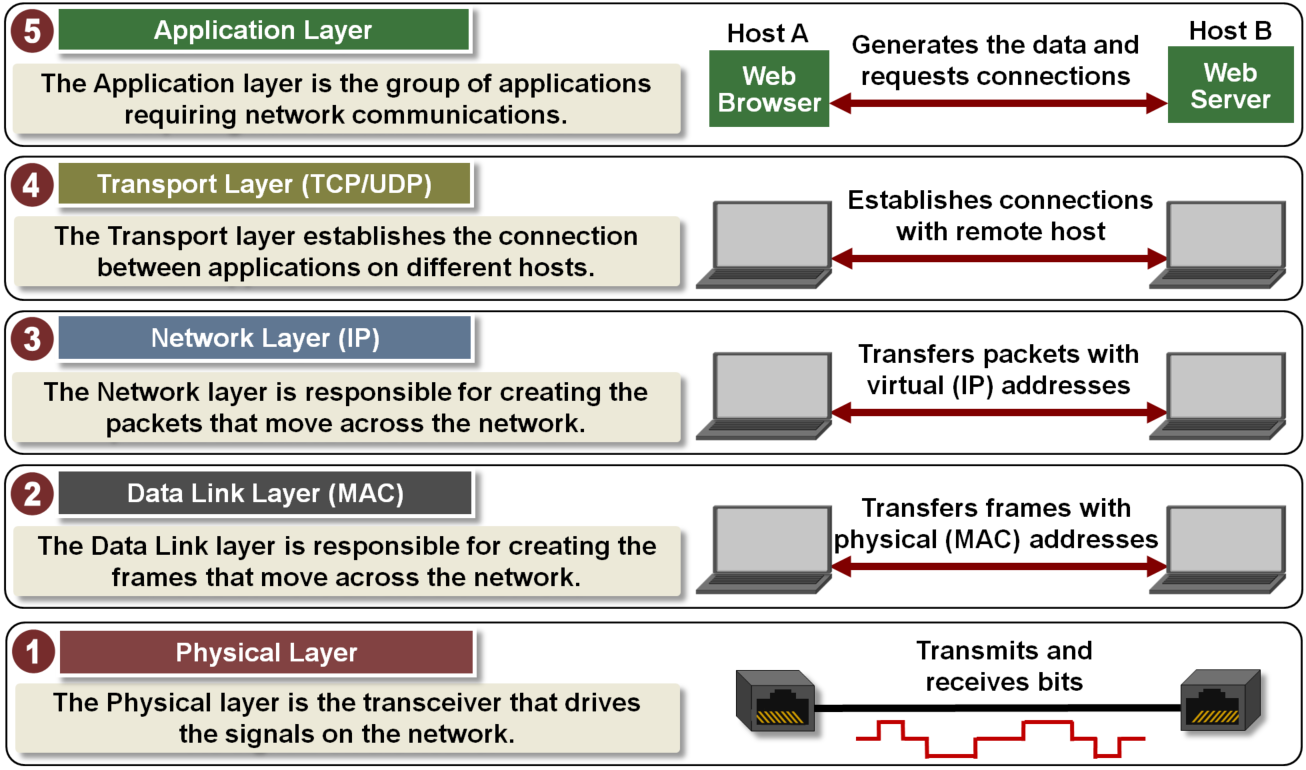
\includegraphics[scale=0.5]{images/5_layer_overview.png}
        \centering
        \caption{Pictorial Layer Summary (bc we all love pictures!)}
    \end{figure}
    
    \begin{description}
        \item[Application Layer] The application layer is where network applications and their application layer protocols reside. The Internet’s application layer includes many protocols, such as the HTTP protocol (which provides for Web document request and transfer), SMTP (which provides for the transfer of e-mail messages), and FTP (which provides for the transfer of files between two end systems). An application-layer protocol is distributed over multiple end systems, with the
        application in one end system using the protocol to exchange packets of information
        with the application in another end system. We’ll refer to this packet of information
        at the application layer as a {\bf message}.
        
        \item[Transport Layer] The Internet’s transport layer transports application-layer messages between
        application endpoints. In the Internet there are two transport protocols, TCP and
        UDP, either of which can transport application-layer messages. TCP provides a
        connection-oriented service to its applications. This service includes guaranteed
        delivery of application-layer messages to the destination and flow control (that is,
        sender/receiver speed matching). TCP also breaks long messages into shorter segments
        and provides a congestion-control mechanism, so that a source throttles its
        transmission rate when the network is congested. The UDP protocol provides a connectionless
        service to its applications. This is a no-frills service that provides no
        reliability, no flow control, and no congestion control. In this book, we’ll refer to a
        transport-layer packet as a {\bf segment}.
        
        \item[Network Layer] The Internet’s network layer is responsible for moving network-layer packets
        known as {\bf datagrams} from one host to another. The Internet transport-layer protocol
        (TCP or UDP) in a source host passes a transport-layer segment and a destination
        address to the network layer, just as you would give the postal service a letter
        with a destination address. The network layer then provides the service of delivering
        the segment to the transport layer in the destination host.
        The Internet’s network layer includes the celebrated IP Protocol, which defines
        the fields in the datagram as well as how the end systems and routers act on these
        fields. There is only one IP protocol, and all Internet components that have a network
        layer must run the IP protocol. The Internet’s network layer also contains routing
        protocols that determine the routes that datagrams take between sources and destinations. The Internet has many routing protocols.
        
        \item[Link Layer] The Internet’s network layer routes a datagram through a series of routers between
        the source and destination. To move a packet from one node (host or router) to the
        next node in the route, the network layer relies on the services of the link layer. In
        particular, at each node, the network layer passes the datagram down to the link
        layer, which delivers the datagram to the next node along the route. At this next
        node, the link layer passes the datagram up to the network layer.
        The services provided by the link layer depend on the specific link-layer protocol
        that is employed over the link. For example, some link-layer protocols provide
        reliable delivery, from transmitting node, over one link, to receiving node. Note that
        this reliable delivery service is different from the reliable delivery service of TCP,
        which provides reliable delivery from one end system to another. Examples of linklayer
        protocols include Ethernet, WiFi, and the cable access network’s DOCSIS protocol.
        As datagrams typically need to traverse several links to travel from source to
        destination, a datagram may be handled by different link-layer protocols at different
        links along its route. For example, a datagram may be handled by Ethernet on one
        link and by PPP on the next link. The network layer will receive a different service
        from each of the different link-layer protocols. In this book, we’ll refer to the linklayer
        packets as {\bf frames}.
        
        \item[Physical Layer] While the job of the link layer is to move entire frames from one network element
        to an adjacent network element, the job of the physical layer is to move the individual
        bits within the frame from one node to the next. The protocols in this layer are
        again link dependent and further depend on the actual transmission medium of the
        link (for example, twisted-pair copper wire, single-mode fiber optics). For example,
        Ethernet has many physical-layer protocols: one for twisted-pair copper wire,
        another for coaxial cable, another for fiber, and so on. In each case, a bit is moved
        across the link in a different way.
    \end{description}
    
    \item[Examples of each layer]$\hfill$
    \begin{enumerate}
            \item[5.] \textbf{Application Layer}: supporting network application (FTP, SMTP, HTTP)
            \item[4.] \textbf{Transport Layer}: process-process data transfer (TCP, UDP)
            \item[3.] \textbf{Network Layer}: routing of datagrams from source to destination (IP, routing 
            protocols)
            \item[2.] \textbf{Link Layer}: data transfer between neighbouring network elements (Ethernet, 
            Wifi, ARP)
            \item[1.] \textbf{Physical Layer}: bits ``on the wire'' (or spectrum)
    \end{enumerate}
    
    
\end{description}

\newpage

\section*{Ch 2. Application Layer}
\noindent
\rule{\linewidth}{0.5mm}
\noindent

\subsection*{Principles of network applications (Section ?.?.?)}

\begin{description}
    \item[Client-Server model] An ``always-on'' \textbf{server} acts as a host, with a permanent IP 
    address, so that a \textbf{client} may intermittently connect with the server. Clients may have
    dynamic IP addresses and communicate only with the server, never between other clients. 
    Processes running in this model are either a client process (one which initiates communication)
    or a server process (one which waits to be contacted).
    
    \item[P2P Architecture] There is no ``always-on server''; peers request service from other peers
    and also provide a service if another peer requests it. They are intermittently connected and
    may change IP addresses. Peers communicate directly with each other. Processes act as a client
    and server process.
\end{description}

\subsection*{Web and HTTP (Section ?.?.?)}

\begin{description}
    \item[Round Trip Time (RTT)] Time for a small packet to travel from the client to the server and
    back.
    
    \item[Non-persistent HTTP] At most one object is sent over a TCP connection, which is then closed
    after it is received. Therefore, downloading multiple objects required multiple connections with 
    the server. When requesting an object, the total time taken $2RTT+\text{file transmission time}$.
    This occurs per object, so when requesting multiple objects, browsers often open parallel TCP
    connections to fetch each.
    
    \item[Persistent HTTP] Multiple objects can be sent over a single TCP connection, as the server
    leaves the connection open after sending its response. A client sends a request as soon as it 
    encounters a referenced object, so as little as $1RTT$ is required for all objects, since the 
    same open connection is used.
    
    \item[HTTP Request]
    A HTTP request message is formatted as
    \begin{align*}
        &\texttt{METHOD REQUEST-URI HTTP-VERSION\textbackslash r\textbackslash n}\\
        &\texttt{REQUEST-HEADER\textbackslash r\textbackslash n}\\
        &\dots\\
        &\texttt{\textbackslash r\textbackslash n}
    \end{align*}
    where $\texttt{METHOD}\in\{\texttt{GET, POST, HEAD}\}$ and
    \begin{align*}
        \texttt{REQUEST-HEADER}\in\{&\texttt{Accept, \dots, Authorization, Expect, From, Host, If-Match,}\\
        &\texttt{If-Modified-Since,\dots, If-Unmodified-since, User-Agent,\dots}\}.
    \end{align*}
    
        \item[HTTP Response]
    A HTTP response message is formatted as
    \begin{align*}
        &\texttt{HTTP-VERSION STATUS-CODE REASON-PHRASE\textbackslash r\textbackslash n}\\
        &\texttt{RESPONSE-HEADER\textbackslash r\textbackslash n}\\
        &\dots\\
        &\texttt{\textbackslash r\textbackslash n}\\
        &\texttt{[message body]}
    \end{align*}
    where \texttt{STATUS-CODE} and \texttt{REASON-PHRASE} are given by
    \begin{enumerate}
        \item[100] Continue
        \item[200] OK
        \item[301] Moved Permanently
        \item[400] Bad Request
        \item[401] Unauthorized
        \item[403] Forbidden
        \item[404] Not Found
        \item[500] Internal Server Error
        \item[502] Bad Gateway
    
        \item[1xx] Informational - Request received, continuing process
        \item[2xx] Success - The action was successfully received, understood, and accepted
        \item[3xx] Redirection - Further action must be taken in order to complete the request
        \item[4xx] Client Error - The request contains bad syntax or cannot be fulfilled
        \item[5xx] Server Error - The server failed to fulfill an apparently valid request
    \end{enumerate}
    among others and 
    \[
        \texttt{RESPONSE-HEADER}\in\{\texttt{Accept-Ranges, Last-Modified, Content-Length, Content-type\dots}\}.
    \]
    
    \item[Cookies] May be used to keep information about the ``state'' between the client and the 
    server. Can be used for authorization, shopping carts, recommendations, etc.
    
    \item[Web Caches] A proxy server may be used to cache common HTTP requests for faster response 
    times. If an object is in the cache, then the proxy server returns it to the requesting client.
    If it is not in the cache, the proxy forwards the request to the server, then forwards the 
    servers response to the client and caches it.
\end{description}

\subsection*{E-mail (Section ?.?)}

\begin{description}
    \item[User Agent] The ``mail reader'' and is used to compose, edit, read, etc mail messages.
    Outgoing and incoming messages are stored on the server. Examples include Outlook, Thunderbird, etc.
    
    \item[Mail server] Contains \textbf{mailbox} of incoming messages for a user and a \textbf{message queue}
    of outgoing (to be sent) mail messages.
    
    \item[Simple Mail Transfer Protocol(SMTP)] for sending messages between mail servers. Uses TCP on
    port 25 as a persistent connection. Contains a handshake, transfer of messages and closure in a
    command/response like interaction.
    
    \item[Mail Access protocols] For retrieving mail from a mail server. Eg POP, IMAP, HTTP.
\end{description}

\subsection*{DNS: Domain Name System (Section ?.?.?)}

\begin{description}
    \item[Services/Structure] Hostname (e.g google.com) to IP address translation. It is implemented
    in a hierarchy of many \textbf{name servers}, which communicate to resolve names (translate).
    There are $13$ logical root name servers world wide, though they are replicated many times.
    
    \item[Top-level domain server (TLD)] Responsible for com, org, net, edu, aero, jobs, museums and 
    all top-level country domains.
    
    \item[Authoritative DNS serves] Organizations own DNS server, providing hostname to IP mappings
    for organizations named hosts.
    
    \item[Local DNS name server] Each ISP may maintain their own. When a DNS request is sent from a 
    host, it is sent to this server. It has a cache of recent requests and acts as a proxy, forwarding
    requests into the hierarchy.
    
    \item[Iterated Query] When the contacted server replies with the name of some other server to 
    contact in order to resolve the request.
    
    \item[Recursive Query] When the contacted server determines the name resolution on its own. It 
    may contact other servers which in turn do this, hence ``recursive.''
    
    \item[Record types] DNS is essentially a distributed database storing resource records (RR) of 
    the form \\
    $(\texttt{name, value, type, ttl})$ where $\texttt{type}\in\{\texttt{A, NS, CNAME, 
    MX}\}$:
    \begin{description}
        \item[A] \texttt{name} is hostname and \texttt{value} is IP address.
        \item[NS] \texttt{name} is domain (foo.com) and \texttt{value} is hostname of authoritative
        name server for this domain
        \item[CNAME] \texttt{name} is alias for some canonical (real) name and \texttt{value} is 
        canocnical name
        \item[MX] \texttt{value} is name of mailserver associated with \texttt{name}.
    \end{description}
    
    \item[DNS format] All DNS packets have the following structure:
    \begin{lstlisting}
        +---------------------+
        | Header              |
        +---------------------+
        | Question            | Question for the name server
        +---------------------+
        | Answer              | Answers to the question
        +---------------------+
        | Authority           |
        +---------------------+
        | Additional          |
        +---------------------+
    \end{lstlisting}
    
    The header describes the type of packet and which fields are contained in the packet. Following
    the header are a number of questions, answers, authority records, and additional records. For
    this project, we will be ignoring the authority and additional fields - your client program must accept
    packets with such fields, but must ignore them.
    Note that a response for a single question may contain multiple answers, such as if an address
    has multiple IP addresses, or if an address has a CNAME and an A record. Your client must process
    the entire answer section and report on each one of these records.
    
    \item[DNS Headers]
    DNS packets have a header that is shown below. Note that requests and replies follow the same header format.
    \begin{lstlisting}
                                    1  1  1  1  1  1
      0  1  2  3  4  5  6  7  8  9  0  1  2  3  4  5
    +--+--+--+--+--+--+--+--+--+--+--+--+--+--+--+--+
    | ID                                            |
    +--+--+--+--+--+--+--+--+--+--+--+--+--+--+--+--+
    |QR|  Opcode   |AA|TC|RD|RA| Z      | RCODE     |
    +--+--+--+--+--+--+--+--+--+--+--+--+--+--+--+--+
    | QDCOUNT                                       |
    +--+--+--+--+--+--+--+--+--+--+--+--+--+--+--+--+
    | ANCOUNT                                       |
    +--+--+--+--+--+--+--+--+--+--+--+--+--+--+--+--+
    | NSCOUNT                                       |
    +--+--+--+--+--+--+--+--+--+--+--+--+--+--+--+--+
    | ARCOUNT                                       |
    +--+--+--+--+--+--+--+--+--+--+--+--+--+--+--+--+
    \end{lstlisting}
    where:
    \begin{description}
        \item[{\tt ID}] A 16 bit identifier assigned by the program that generates any kind of query. This identifier is copied the corresponding reply and can be used by the requester to match up replies to outstanding queries. You should always use 1337 for this field.
        \item[{\tt QR}] A one bit field that specifies whether this message is a query (0), or a response (1).
        \item[{\tt OPCODE}] A four bit field that specifies kind of query in this message.
        \item[{\tt AA}] Authoritative Answer - this bit is only meaningful in responses, and specifies that the responding name server is an authority for the domain name in question section.
        \item[{\tt RD}] Recursion Desired - this bit directs the name server to pursue the query recursively.
        \item[{\tt RA}] Recursion Available - this be is set or cleared in a response, and denotes whether recursive query support is available in the name server. Recursive query support is optional.
        \item[{\tt Z}] Reserved for future use (usually set to 0).
        \item[{\tt RCODE}] Response code - this 4 bit field is set as part of responses.
        \item[{\tt QDCOUNT}] An unsigned 16 bit integer specifying the number of entries in the question section.
        \item[{\tt ANCOUNT}] An unsigned 16 bit integer specifying the number of resource records in the answer section.
        \item[{\tt NSCOUNT}] An unsigned 16 bit integer specifying the number of resource records in the answer section.
        \item[{\tt ARCOUNT}] An unsigned 16 bit integer specifying the number of resource records in the additional records section.
    \end{description}
    
    \item[DNS Questions]
    A DNS question has the format
    \begin{lstlisting}
                                    1  1  1  1  1  1
      0  1  2  3  4  5  6  7  8  9  0  1  2  3  4  5
    +--+--+--+--+--+--+--+--+--+--+--+--+--+--+--+--+
    |                                               |
    / QNAME                                         /
    /                                               /
    +--+--+--+--+--+--+--+--+--+--+--+--+--+--+--+--+
    | QTYPE                                         |
    +--+--+--+--+--+--+--+--+--+--+--+--+--+--+--+--+
    | QCLASS                                        |
    +--+--+--+--+--+--+--+--+--+--+--+--+--+--+--+--+
    \end{lstlisting}
    Where
    
    \begin{description}
        \item[{\tt QNAME}] A domain name represented as a sequence of labels, where each label consists of a length octet followed by that number of octets. The domain name terminates with the zero length octet for the null label of the root.
        \item[{\tt QTYPE}] A two octet code which specifies the type of the query.
        \item[{\tt QCLASS}] A two octet code that specifies the class of the query.
    \end{description}
    
    \item[Attacking DNS] Root and TLD servers may be inundated with traffic in order a denial of 
    service attack. Can also intercept queries from DNS servers and send bogus replies to them, which
    are usually cached.

    \begin{figure}[H]
        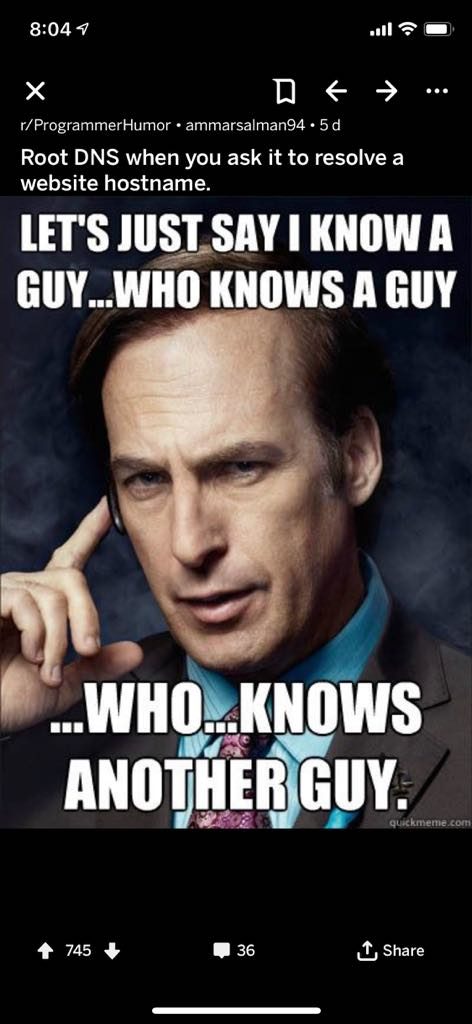
\includegraphics[scale=0.5]{images/dns_summary.jpg}
        \centering
        \caption{Summary of essential DNS concepts}
    \end{figure}    
    
\end{description}

\newpage

\section*{Ch 3. Transport Layer}
\noindent
\rule{\linewidth}{0.5mm}
\noindent

\subsection*{Principles of Transport Layer protocols}

\begin{description}
    \item[Services] Provides logical communication between app processes running on different hosts.
    Sender breaks app message into segments, which are passed to the network layer whereas receiver
    reassembles segments into app message and passes them up to application layer.
    
    \item[Multiplexing] Done at sender-side and handles data from multiple sockets, adding the 
    transport layer header.
    
    \item[Demultiplexing] Done at receiver-side and uses header info to deliver received segments to
    the correct socket. In a connectionless protocol, only the destination port number and IP 
    address is used to determine which socket to send the received data through. In a
    connection-orientated protocol, the source and destination addresses and port numbers are used to
    uniquely identify a socket.
\end{description}

\subsection*{User Datagram Protocol (UDP)}

\begin{description}
    \item[Connectionless] No handshake between sender and receiver; each UDP segment is handled
    independently of others. Segments may be lost or delivered out-of-order, in which case it is up
    to the application to handle this re-request or reorder the segments. Used as there is no handshake
    (meaning no delay), it is simple, small header size and there is no congestion control so segments
    can be sent as fast as desired.
    
    \item[Checksum] Used to detect errors in transmitted segment. A sender computes the checksum by
    treating all data in the datagram (header + payload) as 16bit words and adds them together using
    one's complement sum and puts the result in the ``checksum'' header field. A receiver then adds
    all 16bit values of header and payload: if the result is $0$, no error is detected, else an error
    is detected.
    
    \item[Header] A typical UDP header looks like 
    %TODO include figure
    \begin{lstlisting}
 0      7 8     15 16    23 24    31
+--------+--------+--------+--------+
|     Source      |   Destination   |
|      Port       |      Port       |
+--------+--------+--------+--------+
|                 |                 |
|     Length      |    Checksum     |
+--------+--------+--------+--------+
    \end{lstlisting}
    where 
    \begin{description}
        \item[Source Port] Identifies the sender's port, when used, and should be assumed to be the port
        to reply to if needed. If not used, it should be zero.
        \item[Destination Port] Identifies the receiver's port and is required.
        \item[Length] Specifies the length in bytes of the UDP header and UDP data. The minimum length
        is 8 bytes, the length of the header. The field size sets a theoretical limit of 65,535 bytes
        (8 byte header + 65,527 bytes of data) for a UDP datagram. However the actual limit for the 
        data length, which is imposed by the underlying IPv4 protocol, is 65,507 bytes 
        (65,535 - 8 byte UDP header - 20 byte IP header).
        \item[Checksum] The checksum field may be used for error-checking of the header and data.
        This field is optional in IPv4, and mandatory in IPv6. The field carries all-zeros if unused.
        It is calculated as the 16-bit one's complement of the one's complement sum of a pseudo header
        of information from the IP header, the UDP header, and the data, padded with zero octets at the
        end (if necessary) to make a multiple of two octets.
        \begin{lstlisting}
 0      7 8     15 16    23 24    31
+--------+--------+--------+--------+
|          source address           |
+--------+--------+--------+--------+
|        destination address        |
+--------+--------+--------+--------+
|  zero  |protocol|   UDP length    |
+--------+--------+--------+--------+
        \end{lstlisting}
    \end{description}
\end{description}

\subsection*{Reliable Data Transfer}

\begin{description}
    \item[RDT1.0] Base step for building RDT. Sender will
    \begin{enumerate}
        \item Wait for call from above
        \item Make the segment and send it
        \item Repeat above process
    \end{enumerate}
    Receiver will
    \begin{enumerate}
        \item Wait for call from below
        \item Extract data from segment and push it to above layer
        \item Repeat above process
    \end{enumerate}
    
    \item[RDT2.0] Adds error detection via checksum and feedback via ACK/NAK. Sender will
    \begin{enumerate}
        \item Wait for call from above
        \item Make segment and send it
        \item Wait for response. If response is NAK repeat step, else (ACK received) continue
        \item Repeat above process
    \end{enumerate}
    Receiver will
    \begin{enumerate}
        \item Wait for call from below
        \item If received packet is corrupted send NAK, else extract data and push it to above layer 
        and send ACK
        \item Repeat above process
    \end{enumerate}
    
    \item[RDT2.1] Adds sequence numbers to segments. Sender will
    \begin{enumerate}
        \item Wait for call from above with seq=0
        \item Make segment with seq=0 and send it
        \item Wait for response with ACK or NAK and seq=0. If response is NAK or corrupted repeat last step,
        else continue
        \item Wait for call form above with seq=1
        \item Make segment with seq=1 and send it
        \item Wait for response with ACK or NAK and seq=1. If response is NAK or corrupted repeat last step,
        else continue
        \item Repeat above process
    \end{enumerate}
    Receiver will
    \begin{enumerate}
        \item Wait for call form below with seq=0
        \item If response with has seq=1 send ACK and repeat last step. If response is corrupted send 
        NAK and repeat last step. If response is not corrupted and has seq=0 extract data and push it 
        to above layer and send ACK
        \item Wait for call from below with seq=1
        \item If response with has seq=0 send ACK and repeat last step. If response is corrupted send 
        NAK and repeat last step. If response is not corrupted and has seq=1 extract data and push it 
        to above layer and send ACK
        \item Repeat above process
    \end{enumerate}
    
    \item[RDT2.2] Removes NAK by only sending ACK for last received segment if OK. Sender will
    \begin{enumerate}
        \item Wait for call from above with seq=0
        \item Make segment with seq=0 and send it
        \item Wait for response with ACK and seq=0. If response is corrupted repeat last step,
        else continue
        \item Wait for call form above with seq=1
        \item Make segment with seq=1 and send it
        \item Wait for response with ACK and seq=1. If response is corrupted repeat last step,
        else continue
        \item Repeat above process
    \end{enumerate}
    Receiver will
    \begin{enumerate}
        \item Wait for call form below with seq=0
        \item If response with has seq=1 resend packet and repeat last step. If response is not
        corrupted and has seq=0 extract data and push it to above layer and send ACK
        \item Wait for call from below with seq=1
        \item If response with has seq=0 send ACK and repeat last step. If response is corrupted send 
        NAK and repeat last step. If response is not corrupted and has seq=1 extract data and push it 
        to above layer and send ACK with seq=1
        \item Repeat above process
    \end{enumerate}
    
    \item[RDT3.0] Sender now waits a ``reasonable'' amount of time for ACK. Sender will
    \begin{enumerate}
        \item Wait for call from above with seq=0
        \item Make segment with seq=0, send it and start timer
        \item Wait for response with ACK and seq=0. If response is corrupted do nothing. If timeout occurs, repeat last step else stop timer and continue
        \item Wait for call form above with seq=1
        \item Make segment with seq=1, send it and start timer
        \item Wait for response with ACK and seq=1. If response is corrupted do nothing. If timeout
        occurs, repeat last step else stop timer and continue
        \item Repeat above process 
    \end{enumerate}
    Receiver does not change from RDT2.2.
    
    \item[Pipelining] Window size of $N$ is used to transmit $N$ segments at a time. Only when the
    smallest segment is acked can the window be advanced.
    
    \item[Go-back-N] Sender can have up to $N$ unacked segments in the pipeline and only has timer for
    the last unacked segment. On timeout, the previous $N$ segments are retransmitted. The receiver
    only sends an ACK for the highest received \textit{in-order} segment. If a segment is received
    out of order, it is discarded. An ACK acks all previous segments.
    
    \item[Selective repeat] Receiver \textit{individually} acks all correctly received segments and
    buffers segments as needed for eventual in-order delivery to upper layer. The sender only re-sends
    segments for which it did not receive an ACK.
\end{description}

\subsection*{Transmission Control Protocol (TCP)}

\begin{description}
    \item[Connection-oriented] There is one sender and one receiver per socket. A three-way handshake
    is used to initiate communication between sender and receiver. Provides reliable in-order byte stream,
    flow control and connection management. The sequence number in a TCP header is the byte stream
    number of the first byte in the segments data. The acknowledgement number is the sequence number
    of the next expected byte. 
    
    \item[RTT/Timeouts] RTT is estimated by measuring time from segment transmit until ACK receipt.
    Average RTT is then calculated using previous average and sample taken. That is, 
    $\texttt{NewRTT}=(1-\alpha)\cdot\texttt{OldRTT}+\alpha\cdot\texttt{SampleRTT}.$
    Typical value of $\alpha=0.125$. Timeout is set to be slightly longer than RTT.
    
    \item[Header] A TCP header looks like
    %TODO figure of tcp header. Also explain scaling (e.g. window size)
    \begin{lstlisting}
 0                   1                   2                   3
 0 1 2 3 4 5 6 7 8 9 0 1 2 3 4 5 6 7 8 9 0 1 2 3 4 5 6 7 8 9 0 1
+-+-+-+-+-+-+-+-+-+-+-+-+-+-+-+-+-+-+-+-+-+-+-+-+-+-+-+-+-+-+-+-+
|          Source Port          |        Destination Port       |
+-+-+-+-+-+-+-+-+-+-+-+-+-+-+-+-+-+-+-+-+-+-+-+-+-+-+-+-+-+-+-+-+
|                        Sequence Number                        |
+-+-+-+-+-+-+-+-+-+-+-+-+-+-+-+-+-+-+-+-+-+-+-+-+-+-+-+-+-+-+-+-+
|                     Acknowledgment Number                     |
+-+-+-+-+-+-+-+-+-+-+-+-+-+-+-+-+-+-+-+-+-+-+-+-+-+-+-+-+-+-+-+-+
| Offset|  Res. |     Flags     |             Window            |
+-+-+-+-+-+-+-+-+-+-+-+-+-+-+-+-+-+-+-+-+-+-+-+-+-+-+-+-+-+-+-+-+
|            Checksum           |         Urgent Pointer        |
+-+-+-+-+-+-+-+-+-+-+-+-+-+-+-+-+-+-+-+-+-+-+-+-+-+-+-+-+-+-+-+-+
|                    Options                    |    Padding    |
+-+-+-+-+-+-+-+-+-+-+-+-+-+-+-+-+-+-+-+-+-+-+-+-+-+-+-+-+-+-+-+-+
    \end{lstlisting}
    with
    \begin{description}
        \item[Source Port] Identifies the sending port (16-bits)
        \item[Destination Port] Identifies the receiving port (16-bits)
        \item[Sequence Number] If the SYN flag is set (1), then this is the initial sequence number.
        The sequence number of the actual first data byte and the acknowledged number in the
        corresponding ACK are then this sequence number plus 1. If the SYN flag is clear (0), then this
        is the accumulated sequence number of the first data byte of this segment for the current
        session.
        \item[Acknowledgement Number] If the ACK flag is set then the value of this field is the next
        sequence number that the sender of the ACK is expecting. This acknowledges receipt of all prior
        bytes (if any). The first ACK sent by each end acknowledges the other end's initial sequence
        number itself, but no data.
        \item[Offset] Specifies the size of the TCP header in 32-bit words. 
        \item[Res.] Should be set to 0 (3bits).
        \item[Flags] Contains 9 1bit flags: NS,CWR,ECE,URG,ACK,PSH,RST,SYN,FIN
        \begin{itemize}
            \item[ACK] Indicates that the Acknowledgment field is significant. All packets after the
            initial SYN packet sent by the client should have this flag set.
            \item[SYN] Synchronize sequence numbers. Only the first packet sent from each end should
            have this flag set. Some other flags and fields change meaning based on this flag, and some
            are only valid when it is set, and others when it is clear.
            \item[FIN] Last packet from sender.
        \end{itemize}
        \item[Window Size] The size of the receive window, which specifies the number of window size
        units (by default, bytes) (beyond the segment identified by the sequence number in the
        acknowledgment field) that the sender of this segment is currently willing to receive.
        \item[Checksum] The 16-bit checksum field is used for error-checking of the header, the Payload
        and a Pseudo-Header. The Pseudo-Header consists of the Source IP Address, the Destination IP
        Address, the protocol number for the TCP-Protocol (0x0006) and the length of the TCP-Headers
        including Payload (in Bytes).
        \begin{lstlisting}
+--------+--------+--------+--------+
|           Source Address          |
+--------+--------+--------+--------+
|         Destination Address       |
+--------+--------+--------+--------+
|  zero  |  PTCL  |    TCP Length   |
+--------+--------+--------+--------+
        \end{lstlisting}
    \end{description}
    
    \item[Flow control] The receiver controls how much data the sender sends so as to not overflow the 
    buffer on the receiving end. The TCP window size if the primary tool for doing this.
    
    \item[Congestion control] The sender attempts to limit the amount of data it sends into the network
    so that the performance of the network does not significantly drop. Acknowledgments (or lack thereof)
    are used by sender to infer network conditions between the sender and the receiver.
\end{description}

\newpage

\section*{Ch 4. Network Layer: Data Plane}
\noindent
\rule{\linewidth}{0.5mm}
\noindent

\subsection*{Network Layer}

\begin{description}
    \item[Services] Transports segment from sending to receiving host. Sending side encapsulates 
    segments into datagrams while receiving side delivers segments to transport layer. Network layer
    protocols are in every host/router, which examines header fields in all IP datagrams that pass through.
    
    \item[Data Plane] Local, per router function determining how datagram arriving on router input 
    port should be forwarded to appropriate router output port.
    
    \item[Control Plane] Network-wide logic on how datagrams should be routed among routers along
    end-to-end path from source to destination. 
\end{description}

\subsection*{What's in a Router}

\begin{description}
    \item[Input Port Functions] When a datagram arrives via link layer, the router uses a lookup
    table (forwarding table) to determine which output port to forward the datagram to. Datagrams may
    be queued if arrival rate exceeds that of forwarding rate into switch fabric.
    
    \item[Destination-based Forwarding] Forwarding based only on destination IP address. For example,
    \begin{center}
    \begin{tabular}{l|c}
        Destination address range & Link interface\\
        \hline
        \texttt{1100100 00010111 00010000 00000000} to \texttt{11001000 00010111 00010111 11111111} &  0\\
        \texttt{1100100 00010111 00011000 00000000} to \texttt{11001000 00010111 00011000 11111111} &  1\\
        \texttt{1100100 00010111 00011001 00000000} to \texttt{11001000 00010111 00011001 11111111} &  2\\
        otherwise & 3
    \end{tabular}
    \end{center}
    
    \item[Longest prefix Matching] When looking for forwarding table entry, use the longest address 
    prefix that matches destination address.
    
    \item[Switching fabric] Transfers input buffer to appropriate output buffer. The rate at which 
    this is done is called the \textbf{switching rate} and is often measured as a multiple of 
    input/output line rate. Three types of switching fabric:
    %TODO insert image
    
    \item[Input port queuing] Occurs when switching fabric is slower than all input ports combined.
    Datagram loss may occur upon buffer overflow. Head-of-line (HOL) blocking occurs when queued 
    datagram at front of queue prevents others in queue from moving forward.
    
    \item[Output port functions] Buffers datagrams as switching fabric is usually faster. Datagrams
    are then scheduled to based off of some priority. Recent recommendations on buffering are that
    if there are $N$ flows and a link capacity of $C$, then buffer size should be
    $\frac{\texttt{RTT}\cdot C}{\sqrt N}.$
    
    \item[Scheduling] The process of choosing which datagram to send on a link and which to drop if
    queue becomes full. Different policies include
    \begin{itemize}
        \item FIFO: first in first out
        \item tail drop: drop arriving packets if queue becomes full
        \item priority drop: drop on basis of some priority ordering
        \item random drop: drop randomly
        \item priority scheduling: high priority queue and low priority queue
        \item round robin: cyclically scan multiple classes send one complete packet at a time
        \item weighted fair queue (WFQ): as above, but each class has a weight associated with it
    \end{itemize}
\end{description}

\subsection*{Internet Protocol (IPv4)}

\begin{description}
    \item[Header] A typical IP datagram looks like
    \begin{lstlisting}
 0                   1                   2                   3   
 0 1 2 3 4 5 6 7 8 9 0 1 2 3 4 5 6 7 8 9 0 1 2 3 4 5 6 7 8 9 0 1 
+-+-+-+-+-+-+-+-+-+-+-+-+-+-+-+-+-+-+-+-+-+-+-+-+-+-+-+-+-+-+-+-+
|Version|  IHL  |Type of Service|          Total Length         |
+-+-+-+-+-+-+-+-+-+-+-+-+-+-+-+-+-+-+-+-+-+-+-+-+-+-+-+-+-+-+-+-+
|         Identification        |Flags|      Fragment Offset    |
+-+-+-+-+-+-+-+-+-+-+-+-+-+-+-+-+-+-+-+-+-+-+-+-+-+-+-+-+-+-+-+-+
|  Time to Live |    Protocol   |         Header Checksum       |
+-+-+-+-+-+-+-+-+-+-+-+-+-+-+-+-+-+-+-+-+-+-+-+-+-+-+-+-+-+-+-+-+
|                       Source Address                          |
+-+-+-+-+-+-+-+-+-+-+-+-+-+-+-+-+-+-+-+-+-+-+-+-+-+-+-+-+-+-+-+-+
|                    Destination Address                        |
+-+-+-+-+-+-+-+-+-+-+-+-+-+-+-+-+-+-+-+-+-+-+-+-+-+-+-+-+-+-+-+-+
|                    Options                    |    Padding    |
+-+-+-+-+-+-+-+-+-+-+-+-+-+-+-+-+-+-+-+-+-+-+-+-+-+-+-+-+-+-+-+-+
    \end{lstlisting}
    with
    \begin{description}
        \item[Version] Always 4 for IPv4.
        \item[IHL] The number of 32-bit words. 
        \item[Total Length] the entire packet size in bytes, including header and data. The minimum size
        is 20 bytes (header without data) and the maximum is 65,535 bytes.
        \item[Identification] Used for uniquely identifying the group of fragments of a single IP datagram
        \item[Flags] Reserved (0),DF,MF. If the DF flag is set, and fragmentation is required to route
        the packet, then the packet is dropped. For unfragmented packets, the MF flag is cleared. For
        fragmented packets, all fragments except the last have the MF flag set. The last fragment has a
        non-zero Fragment Offset field, differentiating it from an unfragmented packet.
        \item[Fragmentaiton offset] Measured in units of eight-byte blocks (explained below).
        \item[Time to Live (TTL)] It is specified in seconds, but time intervals less than 1 second are
        rounded up to 1. In practice, the field has become a hop count—when the datagram arrives at a
        router, the router decrements the TTL field by one.
        \item[Protocol] Defines the protocol used in the data portion of the IP datagram.
        \item[Header Checksum]  When a packet arrives at a router, the router calculates the checksum of
        the header and compares it to the checksum field. If the values do not match, the router
        discards the packet. The checksum field is the 16-bit one's complement of the one's complement
        sum of all 16-bit words in the header. For purposes of computing the checksum, the value of the
        checksum field is zero.
        \item[Source Address] IPv4 address of the sender of the packet.
        \item[Destination Address] IPv4 address of the receiver of the packet.
    \end{description}
    
    \item[Fragmentation] Network links have a MTU (largest possible link-level frame). If a packet is
    larger than a links MTU, it must be fragmented. The fragflag is set to 1 and the offset in a 
    packet is the byte of the unfragmented packet divided by $8$.
    
    \item[Addressing] $32$-bit identifier for host/router interface: a router typically has multiple
    interfaces. A subnet is a group of hosts with the same subnet part of IP address which can 
    physically communicate without the router intervening. CIDR notation (Classless InterDomain 
    Routing) defines an address as $a.b.c.d/x$ where $x$ is the number of bits in the subnet part of the
    IP address.
    
    \item[Dynamic Host Configuration Protocol (DHCP)] Allows a host to dynamically obtain an IP address
    from a network server when it joins the network. Typical exchange:
    \begin{enumerate}
        \item Client Broadcast (DHCP discover): is there DHCP server out there?
        \item Server Broadcast (DHCP offer): I am a DHCP server. Here is an IP address you can use.
        \item Client Broadcast (DHCP request): Ok, I'll take that IP address.
        \item Server Broadcast (DHCP ACK): Ok, you have that address.
    \end{enumerate}
    DHCP can also return address of first-hop router for client, name and IP of local DNS server
    and network mask.
    
    \item[Network Address Translation (NAT)] All datagrams leaving a local network have their source
    IP and port replaced to that of the NAT IP and some new port. NAT translation table stores
    (source IP, source port)$\mapsto$(NAT IP, new port) mappings. Incoming datagrams have the NAT IP
    and new port replaced with source IP and source port.
\end{description}

\subsection*{IPv6}

\begin{description}
    \item[Header] A typical IPv6 header looks like
    %TODO insert IPv6 header
    
    \item[Differences from IPv4] IPv6 does not allow for fragmentation en-route, this must be done
    only at the source and destination. The header checksum was also removed as IPv4 contained a TTL
    field, which meant the checksum had to be computed at every hop. 
    
    \item[Tunneling] Not all routers are IPv6 compatible, so the IPv6 datagram is carried as the
    payload of a IPv4 datagram amongst IPv4 routers. 
\end{description}

\newpage

\section*{Ch 5. Network Layer: Control Plane}
\noindent
\rule{\linewidth}{0.5mm}
\noindent

\subsection*{Structure}

\begin{description}
    \item[Per-router control] The traditional approach to structuring the control place, in which 
    individual routing algorithm components in each and every router interact with each other in the
    control plane in order to compute forwarding tables.
    
    \item[Logically centralised control] A distinct (typically remote) controller interacts with local
    control agents (CA) in routers to compute forwarding tables. 
\end{description}

\subsection*{Routing protocols}

\begin{description}
    \item[Link state vector] The topology of the network and link costs are known to all nodes i.e.
    all nodes have the same information. Each node computes its forwarding table by determining the
    ``least costworthy'' (time, no. links used, congestion, etc.) path to all other nodes. One such 
    algorithm is Dijkstra's Algorithm:
    \begin{enumerate}
        \item Let $N'=\{u\}$.
        \item For all nodes $v\neq u$, if $v$ is adjacent to $u$ then set $D(v)=c(u,v)$ else $D(v)=\infty$.
        \item Find $w\notin N'$ such that $D(w)\leq D(v)$ for all nodes $v\notin N'.$
        \item Set $N'=N'\cup\{w\}$.
        \item For all nodes $v\notin N'$ adjacent to $w$, set $D(v)=\min\{D(v), D(w)+c(w,v)\}$.
        \item Repeat steps 3 to 5 untill all nodes are in $N'$.
    \end{enumerate}
    
    \item[Dijkstra’s algorithm]
        See example question
    
    \item[Distance vector] Each router knows only its physically connected neighbours and the link
    costs to those neighbours. Costs are iteratively shared with neighbours and are recomputed when
    new information is made available. If the cost to any other node has changed, then all neighbours 
    are notified. One such algorithm uses the Bellman-Ford equation: let $d_x(y)$ be the cost of the
    least-cost path from $x$ to $y$ and $N$ be the set of all neighbouring nodes to $x.$ Then, 
    $d_x(y)=\min_{v\in N}\{c(x,v)+d_v(y)\}$.
\end{description}

\newpage

\section*{Ch 6. Link Layer}
\noindent
\rule{\linewidth}{0.5mm}
\noindent

\subsection*{Ethernet Frame Structure}
Ethernet frames have the following structure
    \begin{lstlisting}
<- 8 by  ->|<-   6 by    ->|<-   6 by   ->|<-2b->|<-    var   ->|<-4->|
+-+-+-+-+-+-+-+-+-+-+-+-+-+-+-+-+-+-+-+-+-+-+-+-+-+-+-+-+-+-+-+-+-+-+-+
| Preamble |  Dest.Address | Src. Address | Type | ... Data ... | CRC |
+-+-+-+-+-+-+-+-+-+-+-+-+-+-+-+-+-+-+-+-+-+-+-+-+-+-+-+-+-+-+-+-+-+-+-+
    \end{lstlisting}
\begin{description}
    \item[Preamble (8 bytes)] The Ethernet frame begins with an 8-byte preamble field.
    Each of the first 7 bytes of the preamble has a value of 10101010; the last byte is
    10101011. The first 7 bytes of the preamble serve to “wake up” the receiving
    adapters and to synchronize their clocks to that of the sender’s clock.
    
    \item[Destination address (6 bytes)] This field contains the MAC address of the destination
    adapter, BB-BB-BB-BB-BB-BB. When adapter B receives an Ethernet
    frame whose destination address is either BB-BB-BB-BB-BB-BB or the
    MAC broadcast address, it passes the contents of the frame’s data field to the
    network layer; if it receives a frame with any other MAC address, it discards
    the frame.
    
    \item[Source address (6 bytes)] This field contains the MAC address of the adapter that
    transmits the frame onto the LAN, in this example, {\tt AA-AA-AA-AA-AA-AA}.
    
    \item[Type field (2 bytes)] The type field permits Ethernet to multiplex network-layer
    protocols. To understand this, we need to keep in mind that hosts can use other
    network-layer protocols besides IP.
    
    \item[Data field (46 to 1,500 bytes)] This field carries the IP datagram. The maximum
    transmission unit (MTU) of Ethernet is 1,500 bytes. This means that if the IP
    datagram exceeds 1,500 bytes, then the host has to fragment the datagram. The minimum size of the data field is 46 bytes. This means that if the IP datagram is less than 46 bytes, the data field has to be “stuffed” to fill it out to 46 bytes.
    
    \item[Cyclic redundancy check (CRC) (4 bytes)] The purpose
    of the CRC field is to allow the receiving adapter, adapter B, to detect bit
    errors in the frame.
\end{description}

\subsection*{Error Detection and Correction}

\begin{description}
    \item[Single Parity Check] A single bit is added to end of the data in order to make the parity
    \textbf{even}, that is, the number of ones is an even number.
    
    \item[Two-Dimensional Parity Check] Data is arranged in a 2D-array and parity check bits are added
    to the end of each row and column in order to make every row and every column even parity.
    
    \item[Cyclic Redundancy Check (CRC)] $T=2^{n-k}D+R$ where $T$ is the $n$-bit codeword that $D$
    maps to, $D$ is the $k$-bit message/data to send, and $R$ is the remainder of $(2^{n-k}D)/G$, 
    where $G$ is some given generator. In order to check for errors on transmission, divide the received bits 
    by $G$: if the remainder is $0$, then no error is detected. Often, $T,D,R$ and $G$ are written 
    as polynomials where the $i^\text{th}$ bit is the coefficient of the $x^i$ term.
    E.g. $1000011\mapsto x^6+x+1.$ 
    
    \item[Forward Error Correction (FEC)] Correction of detected errors usually requires retransmission,
    which may be costly. FEC attempts to correct any detected errors itself. An error may be corrected
    if there is a codeword $C$ of minimum distance from the received word $T$, where the distance is
    defined to be the number of bits in which two words differ (Hamming distance).
\end{description}

\subsection*{Multiple Access Protocols}

\begin{description}
    \item[Time division multiple access (TDMA)] Each station gets fixed length slot access to channel,
    where the length of time is the time taken to transmit 1 whole packet. Unused slots go idle.
    \item[Frequency division multiple access (FDMA)] Channel spectrum divided into frequency bands and 
    each station is assigned a fixed frequency band. Unused transmission time in frequency bands go idle.
    \item[Slotted ALOHA] When node obtains frame to transmit, transmits in next time slot. If no 
    collision is detected, node can send new frame in next slot, otherwise the node transmits in the 
    next slot with probability $p$ of success. Assuming there are $N$ nodes and each node transmits in a
    slot with probability $p$, the probability any given node transmits successfully is $p(1-p)^{N-1}$.
    Thus, the probability that \textit{any} node has success is $Np(1-p)^{N-1}$. Taking the limit as
    $N\to\infty$, gives maximum efficiency of $\frac1e$.
    \item[Unslotted ALOHA] As above but there is no time synchronization, so a node transmits as soon as
    a frame arrives. The efficiency of this is $\frac1{2e}$.
    \item[Carrier sense multiple access (CSMA)] Nodes listen to channel before transmitting. If it is idle,
    it transmits the entire frame, otherwise transmission is delayed. If a collision occurs, the entire
    frame and transmission time is wasted.
    \item[CSMA/CD (collision detection)] When a collision is detected abort transmission. After aborting,
    node enters \textbf{binary (exponential) backoff}: after $m^\text{th}$ collision, node chooses $K$
    at random from $\{0,1,2,3,dots,2^m-1\}$ and then waits $512K$ bit times to try again. After $10$ or 
    more collisions, $K$ chosen equally randomly from $\{0,1,2,3,\dots,1023\}$.
    \item[Polling] Some ``master'' node invites ``slave'' node to transmit in turn.
    \item[Token passing (round robin)] Token passed from node to node sequentially. Transmit only when
    in possession of node.
\end{description}

\subsection*{LANs}

\begin{description}
    \item[MAC and ARP] MAC addresses used at link layer to send frame ``locally'' from one interface
    to another physically-connected interface (same network, in IP address  sense), consisting of
    48bits. ARP (address resolution protocol) is used to determine an interfaces MAC address, knowing
    its IP address. Each node on LAN keeps an ARP table, which stores (MAC, IP) mappings.
    \item[Routing to another LAN] Sender sends frame to gatway router MAC address but the intended
    recipient's IP address. Router forwards packet, replacing the source MAC with its own and
    destination MAC with that of the receiver (or intermediate router of necessary).
    \item[Ethernet] Traditional topology of LAN was that of a \textbf{bus}, in which all nodes are in 
    the same collision domain. Nowadays the \textbf{star} topology prevails, in which there is an active
    \textbf{switch} in the center of the network. It is a connectionless and unreliable protocol: data
    is only recovered if some higher layer rdt protocol is used (eg.g TCP).
    \item[Ethernet frame] A typical Ethernet frame looks like 
    
    \begin{tabular}[h!]{c|c|c|c|c|c}
    preamble & destination address & source address & type & data & CRC
    \end{tabular}
    
    with
    \begin{description}
        \item[Preamble] 7 bytes of \texttt{10101010} followed by 1 byte of \texttt{10101011} for clock
        synchronization.
        \item[Dest Address] 48bit MAC address. If adapter receives frame with matching or broadcast
        address, passes data to network layer protocol, otherwise the frame is dropped.
        \item[Type] 16bits specifiying the type of frame (Ethernet II or IEEE 802.3)
        \item[Source Address] 48bit MAC address of sender.
        \item[Data] The payload of a packet.
        \item[CRC] Cyclic redundancy check.
    \end{description}
    
    \item[Ethernet switch] Store and forward ethernet frames. Examines the incoming frames' MAC address and
    selectively forwards frame to one or more outgoing links. Uses CSMA/CD to access the segment. Hosts 
    are unaware of of the presence of switches. Switches learn where to send frames dynamically:
    \begin{enumerate}
        \item Record incoming link and MAC address of sending host
        \item Index switch table using MAC destination address
        \item If entry found, forward frame to interface indicated by entry (unless entry is incoming link
        in which case drop the frame) else flood on all other interfaces.
    \end{enumerate}
    
    \item[VLAN] Switch ports are grouped so that a single physical switch can act as multiple virtual 
    switches. Ports can be dynamically be assigned among VLANs. Forwarding between VLANs is done via 
    routing, just as it is with normal LANs/separate switches. VLANs spanning multiple switches must have
    a \textbf{trunk port}, which carries frames in the same VLAN between physical switches. Such frames
    must carry VLAN information, so must use 802.1q protocol. Frames look like
    
    \begin{tabular}{c|c|c|c|c|c|c|c}
    preamble & destination address & source address & tag protocol id & tag control info & type & data & CRC
    \end{tabular}
    
    with changes
    \begin{description}
        \item[Tag protocol identifier] A 16-bit field set to a value of 0x8100 in order to identify the
        frame as an IEEE 802.1Q-tagged frame. This field is located at the same position as the EtherType
        field in untagged frames, and is thus used to distinguish the frame from untagged frames.
        \item[Tag control information] 16bits containing the following:
        \begin{description}
            \item[Priority code point (PCP)] 3bits which refer to the IEEE 802.1p
            class of service and maps to the frame priority level. Different PCP values can be used to
            prioritize different classes of traffic
            \item[Drop eligible indicator (DEI)] 1-bit (formerly CFI) which may be used separately or in
            conjunction with PCP to indicate frames eligible to be dropped in the presence of congestion.
            \item[VLAN identifier (VID)] 12-bits specifying the VLAN to which the frame belongs. The
            hexadecimal values of 0x000 and 0xFFF are reserved. All other values may be used as VLAN
            identifiers, allowing up to 4,094 VLANs. The reserved value 0x000 indicates that the frame does
            not carry a VLAN ID; in this case, the 802.1Q tag specifies only a priority (in PCP and DEI
            fields) and is referred to as a priority tag. On bridges, VID 0x001 (the default VLAN ID) is
            often reserved for a network management VLAN; this is vendor-specific. The VID value 0xFFF is
            reserved for implementation use; it must not be configured or transmitted. 0xFFF can be used to
            indicate a wildcard match in management operations or filtering database entries.
        \end{description}
    \end{description}
\end{description}

\subsection*{Mutliprotocol lable switching (MPLS)}

\begin{description}
    \item[Initial goal] High-speed IP forwarding using a fixed length label instead of the IP address.
    Borrows ideas from virtual circuiting approach.
    
    \item[MPLS capable routers] Forwards packets based only on MPLS label value, however the label value 
    can depend on other information, such as the source address (this is known as traffic engineering).
    This causes packets to the same destination to take different routes. Can also pre-compute backup
    paths in case of link failure for fast re-routing. 
\end{description}

\subsection*{A day in the life of a web request}

\begin{description}
    \item[Connect to internet] DHCP used to get IP address of self, first-hop router and DNS server.
    \item[Gateway Router] Use ARP to get MAC address of first-hop router.
    \item[Get IP address of web server] IP datagram containing DNS request forwarded via LAN to first-hop 
    router. Forwarded over internet to DNS server, which replies with IP addr of web server.
    \item[Connect to web server] Open TCP socket to web server and commence 3-way handshake.
    \item[Request web page] Send HTTP request to web server over HTTP, which sends back an HTTP response.
\end{description}

\newpage

\section*{Ch 8. Security}
\noindent
\rule{\linewidth}{0.5mm}
\noindent

\subsection*{Security Goals}
The following a desirable features of a secure communication link.
\begin{description}
    \item[Confidentiality] Only the sender and intended receiver should be able to understand
        the contents of the transmitted message. Because eavesdroppers may intercept
        the message, this necessarily requires that the message be somehow
        encrypted so that an intercepted message cannot be understood by an interceptor.
        This aspect of confidentiality is probably the most commonly perceived meaning of the term {\it secure communication}.
    \item[Message integrity] We would like to assure any users that the content of their communication
        is not altered, either maliciously or by accident, in transit. Extensions
        to the checksumming techniques that we encountered in reliable transport and
        data link protocols can be used to provide such message integrity.
    \item[End-point authentication] Both the sender and receiver should be able to
        confirm the identity of the other party involved in the communication—
        to confirm that the other party is indeed who or what they claim to be.
    \item[Operational security] Almost all organizations (companies, universities, and
        so on) today have networks that are attached to the public Internet. These networks
        therefore can potentially be compromised. Attackers can attempt
        to deposit worms into the hosts in the network, obtain corporate secrets, map
        the internal network configurations, and launch DoS attacks.
\end{description}

\subsection*{Caesar cipher}
The Caesar cipher (not to be confused with {\it Caesar Salad}) is one of the earliest known and simplest ciphers. It is a type of substitution cipher in which each letter in the plaintext is 'shifted' a certain number of places down the alphabet. For example, with a shift of 1, A would be replaced by B, B would become C, and so on. For example the plain text message \texttt{“bob, i love you. alice”} becomes \texttt{“nkn, sgktc wky. mgsbc.”} when the following cipher is applied:
\begin{align*}
    \text{Plaintext letter:} \, & \quad \texttt{a b c d e f g h i j k l m n o p q r s t u v w x y z} \\
    \text{Ciphertext letter:} \, & \quad \texttt{m n b v c x z a s d f g h j k l p o i u y t r e w q}
\end{align*}

\subsection*{Rail Fence Cipher}
In the rail fence cipher, the plain text is written downwards and diagonally on successive "rails" of an imaginary fence, then moving up when the bottom rail is reached. When the top rail is reached, the message is written downwards again until the whole plaintext is written out. The message is then read off in rows. For example, if 3 "rails" and the message 'WE ARE DISCOVERED. FLEE AT ONCE' is used, the cipherer writes out
\begin{lstlisting}
    W . . . E . . . C . . . R . . . L . . . T . . . E
    . E . R . D . S . O . E . E . F . E . A . O . C .
    . . A . . . I . . . V . . . D . . . E . . . N . .
\end{lstlisting}
We then remove the spaces (.) and read left to right, top to bottom to get the ciphertext
\begin{lstlisting}
    WECRLTEERDSOEEFEAOCAIVDEN
\end{lstlisting}
As an example of solving this cupher we'll use a 3-rail fence to encode a new phrase and include spacing in between the words. Our ciphertext comes out as IA\_EZS\_ELYLK\_UZERLIPL. Note that our ciphertext has a total of 21 units (letters + spaces). This will be important later on as we try to decipher it.\\[1\baselineskip]
To solve the cipher, you must know the height and cycle of the puzzle. The height is simply the number of fence rails used to create it. In this example, we said that 3 fence rails were used, so the height is 3. The height will always be higher than 2 and no more than the number of letters in the ciphertext (in this case 21) or else the phrase will not be properly encoded; the height can thus be discovered by process of elimination if not known.\\[1\baselineskip]
To determine the puzzle width, which will tell us how many total units will be in each row, you must determine the "cycle" of letters. A "cycle" of letters runs from the top row, down through each subsequent row, and then up again, but stopping before reaching the top row again. (The next letter on the top row will actually begin the next cycle.) So a 2-rail puzzle has a "cycle" of 2 letters; a 3-rail puzzle has a "cycle" of 4 letters; a 4-rail puzzle has a "cycle" of 6 letters; etc. (See below.) The math equation for this is: "Cycle" = ([\# of rails] x 2) - 2 (since the top and bottom rows have half as many units per cycle as any middle row(s)).\\[1\baselineskip]
Our 3-rail fence example has a "cycle" of 4 units. So divide the total units (letters + spaces) by the cycle number and round down to the next whole number. There are 21 units in the example, so our "base puzzle width" is 5 (21 / 4 = 5.25, which rounds down to 5). It is important to realize that there are 5 "full cycles" plus a "partial cycle" of 1 more letter (5 x 4 = 20 and 20 + 1 = 21 units). Therefore, the top row has 6 units in it (5 "full cycles" + the 1 extra letter that is starting off the 6th cycle all by itself). The middle row has 10 units (5 "full cycles" x 2 units for each cycle). The bottom row has 5 units (5 "full cycles" x 1 unit for each cycle since it is the bottom-most row).\\[1\baselineskip]
Take the first 6 units from our ciphertext and write them across the top row, leaving much space between the units: {\bf IA\_EZS}\_ELYLK\_UZERLIPL
\begin{lstlisting}
    I . . . A . . . _ . . . E . . . Z . . . S
\end{lstlisting}
The middle row takes the next 10 units and adds 1 unit just after and 1 unit just before each unit in the top row: IA\_EZS{\bf \_ELYLK\_UZE}RLIPL
\begin{lstlisting}
    I . . . A . . . _ . . . E . . . Z . . . S
    . _ . E . L . Y . L . K . _ . U . Z . E .
\end{lstlisting}
The bottom row gets the final 5 units written below and in between the pairs of units in the middle row: IA\_EZS\_ELYLK\_UZE{\bf RLIPL}.
\begin{lstlisting}
    I . . . A . . . _ . . . E . . . Z . . . S
    . _ . E . L . Y . L . K . _ . U . Z . E .
    . . R . . . L . . . I . . . P . . . L . .
\end{lstlisting}
Now just follow the down-up-down-up pattern to determine the original message: I\_REALLY\_LIKE\_PUZZLES!

\subsection*{Firewalls}
A firewall is a combination of hardware and software that isolates an organization’s
internal network from the Internet at large, allowing some packets to pass and blocking
others. A firewall allows a network administrator to control access between the
outside world and resources within the administered network by managing the traffic
flow to and from these resources. A firewall has three goals:
\begin{description}
    \item[All traffic passes through the firewall] A firewall, sits squarely at the boundary between the administered network and the rest of the Internet. While large organizations may use multiple levels of firewalls or distributed firewalls, locating a firewall at a single access point to the network makes it easier to manage and enforce a security-access policy.
    \item[Only authorized traffic, will be allowed to pass] With all traffic entering and leaving the       institutional network passing through the firewall, the firewall can restrict access to authorized      traffic.
    \item[Immune to penetration (if you know what I'm talking about)] The firewall itself is a device       connected to the network. If not designed or installed properly, it can be compromised, in which case it provides only a false sense of security
\end{description}

\subsection*{Intrusion Detection System}
An Intrusion Detection System is a device that generates alerts when it observes potentially malicious traffic. An IDS can be used to detect a wide range of attacks, including network mapping (emanating, for example, from nmap), port scans, TCP stack scans, DoS bandwidth-flooding attacks, worms and viruses, OS vulnerability attacks, and application vulnerability attacks (honestly I have no idea what half of these mean, I just found them in the text book).\\[1\baselineskip]
IDS systems are broadly classified as either {\bf signature-based} systems or
{\bf anomaly-based} systems. A signature-based IDS maintains an extensive database
of attack signatures. Each signature is a set of rules pertaining to an intrusion activity.
A signature may simply be a list of characteristics about a single packet (e.g.,
source and destination port numbers, protocol type, and a specific string of bits in
the packet payload), or may relate to a series of packets. The signatures are normally
created by skilled network security engineers who research known attacks.
An organization’s network administrator can customize the signatures or add its
own to the database.\\[1\baselineskip]
Operationally, a signature-based IDS sniffs every packet passing by it, comparing
each sniffed packet with the signatures in its database. If a packet (or series of
packets) matches a signature in the database, the IDS generates an alert. The alert
could be sent to the network administrator in an e-mail message, could be sent to the
network management system, or could simply be logged for future inspection.
Signature-based IDS systems, although widely deployed, have a number of limitations.
Most importantly, they require previous knowledge of the attack to generate
an accurate signature. In other words, a signature-based IDS is completely blind to
new attacks that have yet to be recorded. Another disadvantage is that even if a signature
is matched, it may not be the result of an attack, so that a false alarm is generated.
Finally, because every packet must be compared with an extensive collection of
signatures, the IDS can become overwhelmed with processing and actually fail to
detect many malicious packets.\\[1\baselineskip]
An anomaly-based IDS creates a traffic profile as it observes traffic in normal
operation. It then looks for packet streams that are statistically unusual, for example,
an inordinate percentage of ICMP packets or a sudden exponential growth in
port scans and ping sweeps. The great thing about anomaly-based IDS systems is
that they don’t rely on previous knowledge about existing attacks—that is, they can
potentially detect new, undocumented attacks. On the other hand, it is an extremely
challenging problem to distinguish between normal traffic and statistically unusual
traffic. To date, most IDS deployments are primarily signature-based, although
some include some anomaly-based features.

\section*{Example Questions}
\noindent
\rule{\linewidth}{0.5mm}
\noindent

\subsection*{Application messages}
Consider the following string of ASCII characters (below) that were captured by Wireshark when the browser sent an HTTP XXX message (i.e., this is the actual content of an HTTP XXX message).
\begin{lstlisting}
GET /index.html HTTP/1.1\r\n
Host: www-net.cs.umass.edu\r\n
User-Agent: Firefox/3.6.10\r\n
Accept: text/html,application/xhtml+xml\r\n
Accept-Language: en-us,en;q=0.5\r\n
Accept-Encoding: gzip,deflate\r\n
Accept-Charset: ISO-8859-1,utf-8;q=0.7\r\n
Keep-Alive: timeout=5, max=1000\r\n
Connection: keep-alive\r\n
\r\n
\end{lstlisting}
The characters \texttt{\textbackslash r\textbackslash n} are carriage return and line-feed characters. Answer the following questions.

\begin{enumerate}
    \item {\it What is the user preference on the “accept-language”?} English, as shown by the \texttt{Accept -Language} field.
    \item {\it Does the server want to bother with persistent connection or not? Why? Or Why not?} Yes, we can see that the server would like to maintain a connection in the \texttt{Connection} field.
    \item {\it Does the browser deal with multiple request/response transaction per connection or not?} No since the connections are kept alive.
\end{enumerate}

\subsection*{Dijkstra's Algorithm}
Given the following graph suppose we would like to find the shortest distance between vertex {\bf A} and each of the other vertices

\begin{figure}[H]
    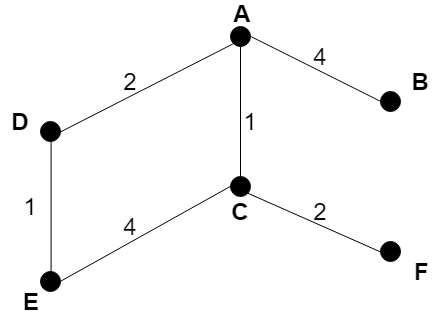
\includegraphics[scale=0.5]{images/COMS_review_dj.png}
    \centering
\end{figure}

To start (iteration $1$) we assume the distance to any other vertex to be infinite and that the shortest distance to {\bf A} is $0$.

\begin{center}
 \begin{tabular}{| c || c |} 
 \hline
 \, & Iter $1$ \\ [0.5ex] 
 \hline\hline
A & $0$ \\ 
 \hline
B & $\infty$ \\
 \hline
C & $\infty$ \\
 \hline
D & $\infty$ \\
 \hline
E & $\infty$ \\
 \hline
F & $\infty$ \\
 \hline
\end{tabular}
\end{center}

With the minimum cost of {\bf A} added to our table we then consider the cost to all the neighbours of {\bf A}. We find that {\bf C} is our least expensive neighbour to {\bf C} with a cost of $1$, so the smallest cost to the vertex {\bf C} is updated and set as $1$. Costs for {\bf B} and {\bf D} that neighbour {\bf A} are also updated but not set as the shortest since only the shortest cost on any iteration is set as the shortest overall path to {\bf A}.

\begin{center}
 \begin{tabular}{| c || c | c |} 
 \hline
 \, & Iter $1$ & Iter $2$ \\ [0.5ex] 
 \hline\hline
A & $0$ & \, \\ 
 \hline
B & $\infty$ & $4$ \\
 \hline
C & $\infty$ & $1$ \\
 \hline
D & $\infty$ & $2$ \\
 \hline
E & $\infty$ & $\infty$ \\
 \hline
F & $\infty$ & $\infty$ \\
 \hline
\end{tabular}
\end{center}

Now that {\bf C} is added we check to see if route costs to {\bf A} are smaller. Indeed since {\bf E} and {\bf F} neighbour {\bf C} the new cost from {\bf E} and {\bf F} to {\bf A} is $5$ and $3$ respectively. On every iteration we check to see if the newly set lowest cost vertex will provide smaller route costs compared to the current route costs.

\begin{center}
 \begin{tabular}{| c || c | c | c |} 
 \hline
 \, & Iter $1$ & Iter $2$ & Iter $3$ \\ [0.5ex] 
 \hline\hline
A & $0$ & \, & \, \\ 
 \hline
B & $\infty$ & $4$ & $4$ \\
 \hline
C & $\infty$ & $1$ & \, \\
 \hline
D & $\infty$ & $2$ & $2$ \\
 \hline
E & $\infty$ & $\infty$ & $5$ \\
 \hline
F & $\infty$ & $\infty$ & $3$ \\
 \hline
\end{tabular}
\end{center}

\begin{center}
 \begin{tabular}{| c || c | c | c | c |} 
 \hline
 \, & Iter $1$ & Iter $2$ & Iter $3$ & Iter $4$ \\ [0.5ex] 
 \hline\hline
A & $0$ & \, & \, & \, \\ 
 \hline
B & $\infty$ & $4$ & $4$ & $4$ \\
 \hline
C & $\infty$ & $1$ & \, & \, \\
 \hline
D & $\infty$ & $2$ & $2$ & \, \\
 \hline
E & $\infty$ & $\infty$ & $5$ & $3$ \\
 \hline
F & $\infty$ & $\infty$ & $3$ & $3$ \\
 \hline
\end{tabular}
\end{center}

\begin{center}
 \begin{tabular}{| c || c | c | c | c | c |} 
 \hline
 \, & Iter $1$ & Iter $2$ & Iter $3$ & Iter $4$ & Iter $5$ \\ [0.5ex] 
 \hline\hline
A & $0$ & \, & \, & \, & \, \\ 
 \hline
B & $\infty$ & $4$ & $4$ & $4$ & $4$ \\
 \hline
C & $\infty$ & $1$ & \, & \, & \, \\
 \hline
D & $\infty$ & $2$ & $2$ & \, & \, \\
 \hline
E & $\infty$ & $\infty$ & $5$ & $3$ & \, \\
 \hline
F & $\infty$ & $\infty$ & $3$ & $3$ & $3$ \\
 \hline
\end{tabular}
\end{center}

\begin{center}
 \begin{tabular}{| c || c | c | c | c | c | c |} 
 \hline
 \, & Iter $1$ & Iter $2$ & Iter $3$ & Iter $4$ & Iter $5$ & Iter $6$ \\ [0.5ex] 
 \hline\hline
A & $0$ & \, & \, & \, & \, & \, \\ 
 \hline
B & $\infty$ & $4$ & $4$ & $4$ & $4$ & $4$ \\
 \hline
C & $\infty$ & $1$ & \, & \, & \, & \, \\
 \hline
D & $\infty$ & $2$ & $2$ & \, & \, & \, \\
 \hline
E & $\infty$ & $\infty$ & $5$ & $3$ & \, & \, \\
 \hline
F & $\infty$ & $\infty$ & $3$ & $3$ & $3$ & \, \\
 \hline
\end{tabular}
\end{center}


\subsection*{Bellman-Ford algorithm}
Given the following graph suppose we would like to find the shortest distance between vertex {\bf A} and each of the other vertices using the Bellman-Ford algorithm
\begin{figure}[H]
    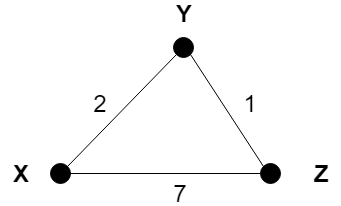
\includegraphics[scale=0.5]{images/COMS_BF_alg.png}
    \centering
\end{figure}
Initially each of the routing tables for our nodes will only display the cost from that node to each of it's neighbours with all other costs assumed to be $\infty$
\begin{figure}[!htb]
   \begin{minipage}{0.3\textwidth}
    %   X-node table
    \centering
     \begin{tabular}{ c | ccc } 
        \, & $x$ & $y$ & $z$ \\
        \hline
        $x$ & 0 & 2 & 7 \\
        $y$ & $\infty$ & $\infty$ & $\infty$ \\
        $z$ & $\infty$ & $\infty$ & $\infty$ \\
    \end{tabular}
    \caption*{Node-X table}
   \end{minipage}
   \begin{minipage}{0.3\textwidth}
    %   Y-node table
    \centering
     \begin{tabular}{ c | ccc } 
        \, & $x$ & $y$ & $z$ \\
        \hline
        $x$ & $\infty$ & $\infty$ & $\infty$ \\
        $y$ & $2$ & $0$ & $1$ \\
        $z$ & $\infty$ & $\infty$ & $\infty$ \\
    \end{tabular}
    \caption*{Node-Y table}
   \end{minipage}
   \begin{minipage}{0.3\textwidth}
    %   Z-node table
    \centering
     \begin{tabular}{ c | ccc } 
        \, & $x$ & $y$ & $z$ \\
        \hline
        $x$ & $\infty$ & $\infty$ & $\infty$ \\
        $y$ & $\infty$ & $\infty$ & $\infty$ \\
        $z$ & $7$ & $1$ & $0$ \\
    \end{tabular}
    \caption*{Node-Z table}
   \end{minipage}
\end{figure}
Each of these nodes then start sharing their distance vector (for example node $x$ will share the distance vector $\left( 0,2,7 \right)$) to each of the other neighbouring nodes. Once the distance vectors have been shared each of the nodes can then start updating their node tables using the Bellman-Ford equation:
\[
    D_{x} = \text{min}_{v} \left\{ c(x,v) + D_{v}(y) \right\}
\]
where $x$ is the starting node and $v$ are each of the nodes neighbouring $v$. In this case $x$ will compute it's new distance to $y$ and $z$ using the distance given by nodes $y$ and $z$. For all other rows it will simply replace these values using the distance vectors from the other nodes. The new distance vector for $x$ is calculated to be
\begin{align*}
    D_{x} (x) &= 0 \\
    D_{x} (y) &= \text{min} \left\{ c(x,y) + D_{y}(y), c(x,z) + D_{z}(y) \right\} = \left\{ 2 + 0, 7 + 1 \right\} = 2 \\
    D_{x} (z) &= \text{min} \left\{ c(x,y) + D_{y}(z), c(x,z) + D_{z}(z) \right\} = \left\{ 2 + 1, 7 + 0 \right\} = 3
\end{align*}
Similar calculations are done for the tables in node $y$ and $z$. The table for the second iteration of this algorithm becomes
\begin{figure}[!htb]
   \begin{minipage}{0.3\textwidth}
    %   X-node table
    \centering
     \begin{tabular}{ c | ccc } 
        \, & $x$ & $y$ & $z$ \\
        \hline
        $x$ & 0 & 2 & 3 \\
        $y$ & $2$ & $0$ & $1$ \\
        $z$ & $7$ & $1$ & $0$ \\
    \end{tabular}
    \caption*{Node-X table}
   \end{minipage}
   \begin{minipage}{0.3\textwidth}
    %   Y-node table
    \centering
     \begin{tabular}{ c | ccc } 
        \, & $x$ & $y$ & $z$ \\
        \hline
        $x$ & $0$ & $2$ & $7$ \\
        $y$ & $2$ & $0$ & $1$ \\
        $z$ & $7$ & $1$ & $0$ \\
    \end{tabular}
    \caption*{Node-Y table}
   \end{minipage}
   \begin{minipage}{0.3\textwidth}
    %   Z-node table
    \centering
     \begin{tabular}{ c | ccc } 
        \, & $x$ & $y$ & $z$ \\
        \hline
        $x$ & $0$ & $2$ & $7$ \\
        $y$ & $2$ & $0$ & $1$ \\
        $z$ & $3$ & $1$ & $0$ \\
    \end{tabular}
    \caption*{Node-Z table}
   \end{minipage}
\end{figure}
With changes to the distance vectors in nodes $x$ and $z$ from our first iteration (the distance vector in $x$ has changed from $\left( 0,2,7 \right)$ to $\left( 0,2,3 \right)$) both nodes again broadcast these updated distance vectors to each of their neighbours. Calculating the distance vector for $x$ in this new iteration we have
\begin{align*}
    D_{x} (x) &= 0 \\
    D_{x} (y) &= \text{min} \left\{ c(x,y) + D_{y}(y), c(x,z) + D_{z}(y) \right\} = \left\{ 2 + 0, 7 + 0 \right\} = 2 \\
    D_{x} (z) &= \text{min} \left\{ c(x,y) + D_{y}(z), c(x,z) + D_{z}(z) \right\} = \left\{ 2 + 1, 3 + 0 \right\} = 3
\end{align*}
Similar calculations are done for the tables in node $z$. The table for the second iteration of this algorithm becomes
\begin{figure}[!htb]
   \begin{minipage}{0.3\textwidth}
    %   X-node table
    \centering
     \begin{tabular}{ c | ccc } 
        \, & $x$ & $y$ & $z$ \\
        \hline
        $x$ & 0 & 2 & 3 \\
        $y$ & $2$ & $0$ & $1$ \\
        $z$ & $3$ & $1$ & $0$ \\
    \end{tabular}
    \caption*{Node-X table}
   \end{minipage}
   \begin{minipage}{0.3\textwidth}
    %   Y-node table
    \centering
     \begin{tabular}{ c | ccc } 
        \, & $x$ & $y$ & $z$ \\
        \hline
        $x$ & $0$ & $2$ & $7$ \\
        $y$ & $2$ & $0$ & $1$ \\
        $z$ & $3$ & $1$ & $0$ \\
    \end{tabular}
    \caption*{Node-Y table}
   \end{minipage}
   \begin{minipage}{0.3\textwidth}
    %   Z-node table
    \centering
     \begin{tabular}{ c | ccc } 
        \, & $x$ & $y$ & $z$ \\
        \hline
        $x$ & $0$ & $2$ & $7$ \\
        $y$ & $2$ & $0$ & $1$ \\
        $z$ & $3$ & $1$ & $0$ \\
    \end{tabular}
    \caption*{Node-Z table}
   \end{minipage}
\end{figure}
Since none of the distance vectors have a new distance vectors, each of the nodes sit and wait until another change in the network topology.



\subsection*{CRC Error-Detection}
In a CRC error-detecting scheme, suppose we choose a generator -of length $r+1$- $g = 110101_{2}$, (which can be represented in polynomial form as $g(x) = x^4 + x^4 + 0 \cdot x^3 + x^2 + 0 \cdot x^1 + x^0 $).
\begin{enumerate}
    \item {\it Encode the bits $D = 1010001101$ You have to show the remainder and the encoded message to send.} For a given piece of data, D, the sender will choose r additional bits, $R$, and append them to $D$ such that the resulting $d + r$ bit pattern (interpreted as a binary number) is exactly divisible by $g$ (i.e., has no remainder) using modulo-2 arithmetic. The process of error checking with CRCs is thus simple: The receiver divides the $d + r$ received bits by $g$. If the remainder is nonzero, the receiver knows that an error has occurred. We can compute $R$ with the formula
    \[
        R = D \cdot 2^r \pmod{g}
    \]
    In this example
    \begin{align*}
        D \cdot 2^r &= 1010001101_{2} \cdot {2^5}_{10} \\
        &= 101000110100000_{2} \\
        &= 20896_{10}
    \end{align*}
    and
    \begin{align*}
        g &= 110101_{2} \\
        &= 53_{10}
    \end{align*}
    So $R = 20896_{10} \pmod{53} = 14_{10} = 01110_{2}$. Thus the data to send is $D = 101000110100000_{2} \; \text{XOR} \; 01110_{2} = 101000110101110_2$. we can use polynomial division in $\mathbb{Z}_2$ to verify our answer.
    \item {\it Suppose the channel introduces two errors in the above-encoded message; i.e., a flip from 1 to 0 or from 0 to 1 in position 1 and 2. What is received? Can the error be detected or not?} Suppose that instead of receiving $D = 101000110101110_2$ from the example above we instead get $D = 011000110101110_2$. To check for corruption we divide $D$ by our chosen generator $g$ using polynomial division (we don't need to keep track of the result). Performing this division we find (subtract top from bottom at each underline):
    \begin{align*}
        110101 |& \, \overline{011000110101110} \\[-10pt]
                & \, \, \underline{110101} \, \text{(shift by 9 bits)} \\[-10pt]
                & \, \, \, 00010010101110 \\[-10pt]
                & \qquad \underline{110101} \\[-10pt]
                & \qquad 01000001110 \\[-10pt]
                & \qquad \, \underline{110101} \\[-10pt]
                & \qquad \, 0101011110 \\[-10pt]
                & \qquad \, \, \underline{110101} \\[-10pt]
                & \qquad \, \, 011111110 \\[-10pt]
                & \qquad \quad \underline{110101} \\[-10pt]
                & \qquad \quad 00101010 \\[-10pt]
                & \qquad \qquad \underline{110101} \\[-10pt]
                & \qquad \qquad 011111 \quad \text{(Remainder)}
    \end{align*}
    Since out remainder is non-zero we can in fact detect the error, since our remainder should be zero.
    
\end{enumerate}

\subsection*{Forward Error Correction (FEC)}
\begin{enumerate}
    \item {\it Find the Hamming Distance between 10000101 and 00011111.} Hamming Distance between two 
    codewords (or message words) is simply the number of bits in which they differ. Mathematically, for
    two words $x=x_0x_1x_2\dots x_n$ and $y=y_0y_1y_2\dots y_n$ where $x_i,y_i\in\{0,1\}$, 
    \[
        d(x,y)=\sum_{i=0}^n (x_i+y_i\mod 2)
    \]
    where $d(x,y)\geq0$. Hence, for this example, the Hamming Distance is $4$.
    
    \item{\it Consider the following maps between message words and codewords for $n=2$ and $k=5$.}
    \begin{align*}
        00&\mapsto00000\\
        01&\mapsto00111\\
        10&\mapsto11001\\
        11&\mapsto11110
    \end{align*}
    \begin{enumerate}
        \item {\it Suppose 00 is sent and error pattern 01010 is introduced in transmission.
        Can this error be detected and/or corrected using FEC?}
        The codeword 00000 is sent however error pattern 01010 is introduced, so 00000+01010=01010 is
        received. This is an invalid codeword, so the error pattern is detected. However, the distance to
        the valid codewords are 2, 3, 3 and 2 respectively. Thus, the pattern cannot be corrected using FEC,
        as there is more than 1 codeword with minimum distance from the received word.
        
        \item {\it Suppose 01 is sent and error pattern 00111 is introduced in transmission.
        Can this error be detected and/or corrected using FEC?}
        The codeword 00111 is sent however error pattern 00111 is introduced, so 00111+00111=00000 is
        received. This is a valid codeword, so the error is not detected using FEC.
        
        \item {\it Suppose 11 is sent and error pattern 00100 is introduced in transmission.
        Can this error be detected and/or corrected using FEC?}
        The codewords 11110 is sent however error pattern 00100 is introduced, so 11110+00100=11010 is
        received. This is an invalid codeword, so the error pattern is detected. Moreover, the distance
        to valid codewords are 3, 4, 2 and 1. Thus, there is a unique codeword that is of minimum distance
        to 11010, so it is corrected to 11110.
    \end{enumerate}
\end{enumerate}

\subsection*{TCP deconstruction}
The following 72 bytes (shown in hexdecimal) are from the packet dump of a TCP packet inside an IP datagram inside an Ethernet frame. Note that unlike a normal Wireshark packet dump, this packet dump {\bf does} include the Ethernet preamble and the Ethernet CRC.
\begin{align*}
    & \texttt{aa aa aa aa aa aa aa ab 00 00 5e 00 01 08 98 90} \\
    & \texttt{96 d8 35 a9 08 00 45 00 00 28 41 71 40 00 80 06} \\
    & \texttt{00 00 0a 21 02 98 d0 5c ec 52 e1 75 00 50 e7 3e} \\
    & \texttt{50 0c 1b a0 80 d4 50 11 f7 39 c9 82 00 00 00 00} \\
    & \texttt{00 00 00 00 c8 aa ab cd}
\end{align*}
Complete each of the following fields of the various protocol layers (in the
indicated format).\\[1\baselineskip]
Recall from the ethernet section that our IP datagram is cushioned by $22$ bytes on the left (consisting of preamble, dest addr, src addr and type) and $4$ bytes on the right (just the CRC check). Also the IP datagram headers take up the first $20$ bytes (assuming no options are given) of the data inside the ethernet frame, thus the bytes that make up our our ethernet frame are
\begin{align*}
    & \texttt{aa aa aa aa aa aa aa ab 00 00 5e 00 01 08 98 90} \\
    & \texttt{96 d8 35 a9 08 00}
\end{align*}
the bytes that make up our IP header are
\begin{align*}
    & \texttt{45 00 00 28 41 71 40 00 80 06 00 00 0a 21 02 98} \\
    & \texttt{d0 5c ec 52}
\end{align*}
Everything between the IP header and the CRC check will be our TCP datagram. Thus the bytes that make up our TCP are
\begin{align*}
    & \texttt{e1 75 00 50 e7 3e 50 0c 1b a0 80 d4 50 11 f7 39} \\
    & \texttt{c9 82 00 00 00 00 00 00 00 00}
\end{align*}
For easy reference here are IP header and TCP datagram structures:
\begin{figure}[H]
    \centering
    \caption{Ethernet frame structure}
    \begin{lstlisting}
|<- 8 by ->|<-   6 by    ->|<-   6 by   ->|<-2b->|<-    var   ->|<-4->|
+-+-+-+-+-+-+-+-+-+-+-+-+-+-+-+-+-+-+-+-+-+-+-+-+-+-+-+-+-+-+-+-+-+-+-+
| Preamble |  Dest.Address | Src. Address | Type | ... Data ... | CRC |
+-+-+-+-+-+-+-+-+-+-+-+-+-+-+-+-+-+-+-+-+-+-+-+-+-+-+-+-+-+-+-+-+-+-+-+
    \end{lstlisting}
\end{figure}
\begin{figure}[H]
    \centering
    \caption{IP header structure}
    \begin{lstlisting}
 0                   1                   2                   3   
 0 1 2 3 4 5 6 7 8 9 0 1 2 3 4 5 6 7 8 9 0 1 2 3 4 5 6 7 8 9 0 1 
+-+-+-+-+-+-+-+-+-+-+-+-+-+-+-+-+-+-+-+-+-+-+-+-+-+-+-+-+-+-+-+-+
|Version|  IHL  |Type of Service|          Total Length         |
+-+-+-+-+-+-+-+-+-+-+-+-+-+-+-+-+-+-+-+-+-+-+-+-+-+-+-+-+-+-+-+-+
|         Identification        |Flags|      Fragment Offset    |
+-+-+-+-+-+-+-+-+-+-+-+-+-+-+-+-+-+-+-+-+-+-+-+-+-+-+-+-+-+-+-+-+
|  Time to Live |    Protocol   |         Header Checksum       |
+-+-+-+-+-+-+-+-+-+-+-+-+-+-+-+-+-+-+-+-+-+-+-+-+-+-+-+-+-+-+-+-+
|                       Source Address                          |
+-+-+-+-+-+-+-+-+-+-+-+-+-+-+-+-+-+-+-+-+-+-+-+-+-+-+-+-+-+-+-+-+
|                    Destination Address                        |
+-+-+-+-+-+-+-+-+-+-+-+-+-+-+-+-+-+-+-+-+-+-+-+-+-+-+-+-+-+-+-+-+
|                    Options                    |    Padding    |
+-+-+-+-+-+-+-+-+-+-+-+-+-+-+-+-+-+-+-+-+-+-+-+-+-+-+-+-+-+-+-+-+
    \end{lstlisting}
\end{figure}
\begin{figure}[H]
    \centering
    \caption{TCP datagram structure}
    \begin{lstlisting}
 0                   1                   2                   3
 0 1 2 3 4 5 6 7 8 9 0 1 2 3 4 5 6 7 8 9 0 1 2 3 4 5 6 7 8 9 0 1
+-+-+-+-+-+-+-+-+-+-+-+-+-+-+-+-+-+-+-+-+-+-+-+-+-+-+-+-+-+-+-+-+
|          Source Port          |        Destination Port       |
+-+-+-+-+-+-+-+-+-+-+-+-+-+-+-+-+-+-+-+-+-+-+-+-+-+-+-+-+-+-+-+-+
|                        Sequence Number                        |
+-+-+-+-+-+-+-+-+-+-+-+-+-+-+-+-+-+-+-+-+-+-+-+-+-+-+-+-+-+-+-+-+
|                     Acknowledgment Number                     |
+-+-+-+-+-+-+-+-+-+-+-+-+-+-+-+-+-+-+-+-+-+-+-+-+-+-+-+-+-+-+-+-+
| Offset|  Res. |     Flags     |             Window            |
+-+-+-+-+-+-+-+-+-+-+-+-+-+-+-+-+-+-+-+-+-+-+-+-+-+-+-+-+-+-+-+-+
|            Checksum           |         Urgent Pointer        |
+-+-+-+-+-+-+-+-+-+-+-+-+-+-+-+-+-+-+-+-+-+-+-+-+-+-+-+-+-+-+-+-+
|                    Options                    |    Padding    |
+-+-+-+-+-+-+-+-+-+-+-+-+-+-+-+-+-+-+-+-+-+-+-+-+-+-+-+-+-+-+-+-+
    \end{lstlisting}
\end{figure}
Armed with this knowledge we can now produce the following information.
\begin{enumerate}
    \item {\it Ethernet Source Address. (Hexadecimal)} The Ethernet source address is located at the start of the $14^{th}$ byte in the Ethernet header. We can read this value off as $989096d835a9_{16}$
    \item {\it Ethernet Destination Address. (Hexadecimal)} We can read this value off as $00005e000108_{16}$
    \item {\it IP Source Address. (Dotted Decimal)} Read at the beginning of the $12^{th}$ byte in of IP header bytes as $0a.21.02.98_{16} = 10.33.2.152_{10}$
    \item {\it IP Destination Address. (Dotted Decimal)}  Read at the beginning of the $16^{th}$ byte in of IP header bytes as $d0.5c.ec.52_{16} = 13.92.236.82_{10}$
    \item {\it TCP Source Port. (Decimal)} Read off the first two bytes of the TCP datagram bytes as $e175_{16} = 57717_{10}$
    \item {\it TCP Destination Port. (Decimal)} Read off the next two bytes of the TCP datagram bytes as $0050_{16} = 80_{10}$
    \item {\it IP Version. (Decimal)} Upper four bits of $45_{16}$ which is $4_{16} = 4_{10}$.
    \item {\it IP Header Length in bytes. (Decimal)} This is appears as IHL in the structure. Read off as $5_{16} = 5_{10}$, but this value needs to be multiplied by $4$ to give the true header length, so the answer is $20$ bytes (standard header size).
    \item {\it Datagram Length in bytes. (Decimal)} Read off as $28_{16} = 40_{10}$.
    \item {\it TCP Flags. (Binary)} TCP flags have the following structure - \texttt{Reserved (three bits) | Not set | Congestion Window | ECN-Echo | Urgent | Ack | Push | Reset | Syn | Fin } -. The corresponding values are given as $11_{16} = 000000010001_{2}$ now we we can give the values for the following flags
    \begin{description}
        \item[URG Flag] $0$
        \item[ACK Flag] $1$
        \item[PSH Flag] $0$
        \item[RST Flag] $0$ (Reset)
        \item[SYN Flag] $0$
        \item[FIN Flag] $1$
    \end{description}
    \item {\it TCP Sequence Number. (Hexademical)} Read as $e73e500c_{16}$
    \item {\it TCP Acknowledgement Number. (Hexademical)} Read as $1ba080d4_{16}$
    \item {\it IP Header Checksum. (Hexademical)} Read as $0a21_{16}$
    \item {\it TCP Internet Checksum. (Hexademical)} Read as $c982_{16}$
    \item {\it Ethernet CRC. (Hexademical)} Read as $c8aaabcd_{16}$ (Last $4$ bytes of hex dump).
\end{enumerate}


\subsection*{Checksum}
Take the following truncated excerpt of an IPv4 packet. The header is shown in bold and the checksum is underlined.
\begin{align*}
    \texttt{{\bf 4500 0073 0000 4000 4011 \underline{b861} c0a8 0001}} \\
    \texttt{{\bf c0a8 00c7} 0035 e97c 005f 279f 1e4b 8180}\\
\end{align*}
Find and backwards check the IPv4 checksum.\\[1\baselineskip]
The header checksum is computed by treating each 2 bytes in the header as a number and summing these numbers using 1s complement arithmetic. A carry check and correction can be performed with each addition or as a post-process after all additions. If another carry is generated by the correction, another 1 is added to the sum. To calculate the checksum, we can first calculate the sum of each 16 bit value within the header, skipping only the checksum field itself.
\[
    4500_{16} + 0073_{16} + 0000_{16} + 4000_{16} + 4011_{16} + c0a8_{16} + 0001_{16} + c0a8_{16} + 00c7_{16} = 2479c_{16}
\]
The first digit is the carry count and is added to the sum:
\[
    2_{16} + 479c_{16} = 479e_{16}
\]
To obtain the checksum we take the one's complement of this result
\begin{align*}
    \overline{479e_{16}} = \overline{0100011110011110_{2}} = 1011100001100001_{2} = b861_{16}
\end{align*}
When verifying a checksum, the same procedure is used as above, except that the original header checksum is not omitted.
\begin{align*}
    4500_{16} + 0073_{16} + 0000_{16} + 4000_{16} + 4011_{16} + b861_{16} + c0a8_{16} + 0001_{16} + c0a8_{16} + 00c7_{16} = 2fffd_{16}
\end{align*}
Add the carry bits:
\begin{align*}
    fffd_{16} + 2_{16} = ffff_{16}
\end{align*}
Taking the ones' complement (flipping every bit) yields 0000, which indicates that no error is detected. IP header checksum does not check for the correct order of 16 bit values within the header. \\[3\baselineskip]
If the Internet (Protocol) checksum method is adopted, what message will be sent if data is \texttt{5BBCEF35}? If the message received is  \texttt{5BBC EF35 B3F3}, will the message be accepted or dropped? (Show your working.)\\[1\baselineskip]
Similar to the first question we can add together the 2-byte blocks using one's complement.
\begin{align*}
    5bbc_{16} + ef35_{16} = 14af1_{16}
\end{align*}
Again we add the carry of $1$ to our sum to get $4af1_{16} + 1_{16} = 4af2_{16}$. Finally we need to take the one's complement of this result to get our final check sum.
\begin{align*}
    \overline{}{4af2_{16}} = \overline{0100101011110010_{2}} = 1011010100001101_{2} = b50d_{16}
\end{align*}
This also means that the message being received shall be dropped since the payload and checksum do not match.

\end{document}
